% !TeX program = lualatex
% !BIB program = biber

\documentclass[a4paper,14pt,russian]{extreport}

\usepackage{polyglossia}
\setmainlanguage[babelshorthands = true]{russian}
\setotherlanguage{english}

%\usepackage{newtxmath}
\usepackage[no-math]{fontspec}

\defaultfontfeatures{Ligatures = TeX, Mapping = tex-text}

\setmainlanguage[babelshorthands = true]{russian}
\setotherlanguage{english}

\setmainfont{Times New Roman}

\newfontfamily\cyrillicfont{Times New Roman}
\newfontfamily\englishfont{Times New Roman}

\newfontfamily\cyrillicfonttt{Courier New}[Script=Cyrillic]
\newfontfamily\englishfonttt{Courier New}

\usepackage[
left=30mm,
right=10mm, 
top=20mm,
bottom=20mm,
]{geometry}

\makeatletter
	\renewcommand\LARGE{\@setfontsize\LARGE{22pt}{20}}
	\renewcommand\Large{\@setfontsize\Large{20pt}{20}}
	\renewcommand\large{\@setfontsize\large{16pt}{20}}
\makeatother

\usepackage{microtype} % Настройка переносов
\sloppy

\usepackage{setspace} % Настройка межстрочного интервала
\onehalfspacing

\usepackage{indentfirst} % Настройка абзацного отступа
\setlength{\parindent}{12.5mm}

\usepackage[unicode,hidelinks]{hyperref}
\usepackage{xifthen}

\usepackage{colortbl}

\usepackage[normalem]{ulem}
% Текст под линией 
\newcommand*{\undertext}[2]{%
	\begin{tabular}[t]{@{}c@{}}%
		#1\\\relax\scriptsize(#2)%
	\end{tabular}
}

% горизонтальная линия
\makeatletter
\newcommand{\vhrulefill}[1]
{
	\leavevmode\leaders\hrule\@height#1\hfill \kern\z@
}

\usepackage[figure,table]{totalcount} % Подч изображений, таблиц
\usepackage{rotating} % Поворот изображения вместе с названием
\usepackage{lastpage} % Для подсчета числа страниц

\usepackage{titlesec}
\usepackage{titletoc}
\usepackage{tocloft}
\usepackage{pdfpages}

\setcounter{tocdepth}{5}

\setlength{\cftbeforetoctitleskip}{-25pt}
\renewcommand{\cfttoctitlefont}{\large\bfseries}

\renewcommand{\cftchapfont}{\large\bfseries}
\renewcommand{\cftsecfont}{\large}
\renewcommand{\cftchapleader}{\cftdotfill{\cftdotsep}}
\renewcommand{\cftpartleader}{\cftdotfill{\cftdotsep}}

\setlength{\cftbeforepartskip}{10pt}


\makeatletter
\renewcommand{\toclevel@part}{0}
\renewcommand{\toclevel@chapter}{0}
\renewcommand{\toclevel@section}{1}
\renewcommand{\toclevel@subsection}{2}
\makeatother
\usepackage{bookmark}

\setcounter{secnumdepth}{5}

\titleformat{\part}[block]
{\large\bfseries}{\hspace{12.5mm}\thechapter}{0.5em}{\large\centering}

\titleformat{\chapter}[block]
{\large\bfseries}{\hspace{12.5mm}\thechapter}{0.5em}{\large\raggedright}

\titleformat{\section}[block]
{\large\bfseries}{\hspace{12.5mm}\thesection}{0.5em}{\large\raggedright}
\renewcommand{\thesection}{\arabic{chapter}.\arabic{section}} 

\titleformat{\subsection}[block]
{\large\bfseries}{\hspace{12.5mm}\thesubsection}{0.5em}{\large\raggedright}
\renewcommand{\thesubsection}{\arabic{chapter}.\arabic{section}.\arabic{subsection}}

\titleformat{\subsubsection}[block]
{\large\bfseries}{\hspace{12.5mm}\thesubsubsection}{0.5em}{\large\raggedright}
\renewcommand{\thesubsubsection}{\arabic{chapter}.\arabic{section}.\arabic{subsection}.\arabic{subsubsection}}

\titleclass{\part}{top}
\titlespacing*{\part}{12.5mm}{-22pt}{10pt}

\titlespacing{\chapter}{0pt}{-22pt}{10pt}
\titlespacing{\section}{0pt}{10pt}{10pt}
\titlespacing{\subsection}{0pt}{10pt}{10pt}
\titlespacing{\subsubsection}{0pt}{10pt}{10pt}

% ---------------------------------------- CAPTION --------------------------------- %

\usepackage[
	labelsep=endash,
	singlelinecheck=false,
]{caption}

\captionsetup[figure]{justification=centering, name=Рисунок}
\captionsetup[table]{justification=raggedleft}
\captionsetup[listing]{justification=raggedright}


% ---------------------------------------- ABBRS --------------------------------- %

\usepackage{enumitem}
\newcounter{descriptcount}
\newlist{enumdescript}{description}{2}
\setlist[enumdescript,1]{
	leftmargin=\parindent,
	itemindent=5pt,
	labelsep=0.25em,
	align=left,
	parsep=0pt,
	itemsep=0pt,
	topsep=0pt,
	before={\setcounter{descriptcount}{0}
		\renewcommand*\thedescriptcount{\arabic{descriptcount})}
		\setlength{\parindent}{12.5mm}},
	font=\normalfont\stepcounter{descriptcount}\thedescriptcount~
}
\setlist[enumdescript,2]{
	before={\setcounter{descriptcount}{0}
		\renewcommand*\thedescriptcount{\roman{descriptcount}.}}
	,font=\normalfont\stepcounter{descriptcount}\thedescriptcount~
}

\def\labelitemi{---} % Изменение буллета для списков
\setlist[itemize]{
	leftmargin=\parindent,
	itemindent=0pt,
	labelwidth=15pt,
	labelsep=2.5mm,
	labelindent=\dimexpr\parindent-10mm-2.5mm\relax,
	align=left,
	parsep=0pt,
	itemsep=0pt,
	topsep=0pt,
	before={\setlength{\parindent}{12.5mm}}
}

\setlist[enumerate]{
	leftmargin=\parindent,            % убираем стандартный отступ списка
	itemindent=0pt,     % основной текст начинается с красной строки
	labelwidth=10pt,           % выделяем место для номера
	labelsep=2.5mm,            % отступ между номером и текстом
	labelindent=\dimexpr\parindent-10mm-2.5mm\relax, % позиция номера (левее красной строки)
	align=left,
	parsep=0pt,
	itemsep=0pt,
	topsep=0pt,
	label=\arabic*),
	before={\setlength{\parindent}{12.5mm}}
}


% ---------------------------------------- TABLE  ----------------------------------------

\usepackage{xcolor}
\usepackage{tabularx}
\usepackage{booktabs}
\usepackage{multirow}
\usepackage{diagbox}
\usepackage{placeins}

\newcolumntype{O}{>{\centering\arraybackslash}p{0.08\textwidth}}
\newcolumntype{T}{>{\centering\arraybackslash}p{0.3\textwidth}}
\newcolumntype{L}{>{\centering\arraybackslash}p{0.45\textwidth}}
\newcolumntype{P}{>{\centering\arraybackslash}p{0.2\textwidth}}
\newcolumntype{R}{>{\centering\arraybackslash}p{0.22\textwidth}}
\newcolumntype{F}{>{\centering\arraybackslash}p{0.25\textwidth}}
\newcolumntype{S}{>{\centering\arraybackslash}p{0.15\textwidth}}
\newcolumntype{B}{>{\centering\arraybackslash}p{0.12\textwidth}}
\newcolumntype{U}{>{\centering\arraybackslash}p{0.16\textwidth}}
\newcolumntype{N}{>{\centering\arraybackslash}p{0.19\textwidth}}
\newcolumntype{H}{>{\centering\arraybackslash}p{0.13\textwidth}}
\newcolumntype{E}{>{\centering\arraybackslash}p{0.18\textwidth}}
\newcolumntype{G}{>{\centering\arraybackslash}p{0.6\textwidth}}
\newcolumntype{Q}{>{\centering\arraybackslash}p{0.1\textwidth}}
\newcolumntype{A}{>{\centering\arraybackslash}p{0.5\textwidth}}

% ---------------------------------------- FIGURE ----------------------------------------

\usepackage{graphicx}
\usepackage{float}
\usepackage{wrapfig}
\usepackage{tikzscale}
\usepackage{tikz}
\usetikzlibrary{calc}
\usetikzlibrary{shapes.misc}      % Для 'rounded rectangle'
\usetikzlibrary{shapes.geometric} % Для 'diamond'
\usetikzlibrary{positioning}      % Для синтаксиса 'below=of'
\usetikzlibrary{arrows.meta}      % Для более точного определения стрелок
\usepackage[notransparent]{svg}
\svgpath{{images/}}
\makeatletter
	\let\quote@name\unquote@name
\makeatother


\usepackage{pgfplots}
\pgfplotsset{compat=newest}

% ----------------------------------------- MATH -----------------------------------------

\usepackage{lscape}
\usepackage{afterpage}

\usepackage{amsmath}

\DeclareMathOperator*{\argmax}{arg\,max}
\DeclareMathOperator*{\argmin}{arg\,min}
% ----------------------------------------- LST -----------------------------------------
\usepackage{listings}
\usepackage{courier}
\usepackage{spverbatim}

\renewcommand{\lstlistingname}{Листинг}

\newcommand{\codefont}{\fontfamily{pcr}}
\newcommand{\keywordsfont}{\fontfamily{pcr}\bfseries}

%\usepackage{minted}
\lstset{
	basicstyle=\codefont\footnotesize,
	keywordstyle=\keywordsfont\color{black},
	numbers=left,
	numberstyle=\fontfamily{pcr}\tiny,
	showstringspaces=false,
	numbersep=10pt,
	tabsize=4,
	frame=tblr, 
	xleftmargin=25pt,
	framexleftmargin=18pt,
	framexrightmargin=-5pt,
	% framexbottommargin=10pt,
	% linewidth=0.95\pagewidth,
	float=H, % Makes listings float
	floatplacement=!ht, % Prevents listings from breaking across pages
	aboveskip=0pt, % Adds space above
	belowskip=0pt,
	breaklines=true,
	extendedchars=true,
	texcl=true,
	inputencoding=utf8,
	basicstyle=\cyrillicfonttt\footnotesize,
	columns=flexible,  % Гибкое распределение ширины столбцов
	keepspaces=true,   % Сохранять пробелы как есть
	basewidth={0.5em,0.5em}  % Настройка базовой ширины символов
}

\usepackage[ruled,linesnumbered,resetcount,algochapter]{algorithm2e}
\SetKwInput{KwData}{Исходные параметры}
\SetKwInput{KwResult}{Результат}
\SetKwInput{KwIn}{Входные данные}
\SetKwInput{KwOut}{Выходные данные}
\SetKwIF{If}{ElseIf}{Else}{если}{тогда}{иначе если}{иначе}{конец условия}
\SetKwFor{While}{до тех пор, пока}{выполнять}{конец цикла}
\SetKw{KwTo}{от}
\SetKw{KwRet}{возвратить}
\SetKw{Return}{возвратить}
\SetKwBlock{Begin}{начало блока}{конец блока}
\SetKwSwitch{Switch}{Case}{Other}{Проверить значение}{и выполнить}{вариант}{в противном случае}{конец варианта}{конец проверки значений}
\SetKwFor{For}{цикл}{выполнять}{конец$\;$цикла} % очевидный и невероятный костыль
\SetKwFor{ForEach}{для каждого}{выполнять}{конец цикла}
\SetKwRepeat{Repeat}{повторять}{до тех пор, пока}
\SetAlgorithmName{Листинг}{алгоритм}{Список алгоритмов}

% ----------------------------------------- BIBLIO ---------------------------------------
\usepackage{totcount}
\regtotcounter{table}    % для подсчета таблиц
\newcounter{citnum}
\regtotcounter{citnum}
\newtotcounter{appendix}  % создаем счетчик приложений


\usepackage[
	backend=biber,
	style=gost-numeric,
	language=auto,
	sorting=none,
	maxnames=999,
	doi=false,
	isbn=false,
	url=true,
	dashed=false
]{biblatex}

\makeatletter
\AtEveryBibitem{\stepcounter{citnum}}
\makeatother

% Базовые настройки
\usepackage{csquotes}
\addbibresource{ref-lib.bib}

% Настройка формата элементов
\DeclareFieldFormat{title}{%
	\ifentrytype{misc}{%
		#1 [Электронный ресурс]%
	}{%
		\ifentrytype{article}{%
			#1 [Электронный ресурс]%
		}{%
			#1%
		}%
	}%
}
\DeclareFieldFormat{url}{Режим доступа: #1}
\DeclareFieldFormat{urldate}{(дата обращения: \ifnum\thefield{urlday}<10 0\fi\thefield{urlday}.\ifnum\thefield{urlmonth}<10 0\fi\thefield{urlmonth}.\thefield{urlyear})}

% Настройка URL
\usepackage{url}
\urlstyle{same}



\addbibresource{ref-lib.bib}

\begin{document}
	\renewcommand{\contentsname}{\centerline{СОДЕРЖАНИЕ}}
	
	%\begin{titlepage}
	
	\centering
	
	\begin{wrapfigure}[7]{l}{0.14\linewidth}
		\vspace{3.4mm}
		\hspace{-8mm}
		
\includegraphics[width=1\linewidth]{images/bmstu_logo.png}
	\end{wrapfigure}
	
	{
		\singlespacing \small \fontseries{b}\selectfont
		Министерство науки и высшего образования Российской Федерации \\
		Федеральное государственное бюджетное образовательное учреждение \\
		высшего образования \\
		<<Московский государственный технический университет \\
		имени Н.~Э.~Баумана \\
		(национальный исследовательский университет)>> \\
		(МГТУ им. Н.~Э.~Баумана) \\
	}
	
	\vspace{-4.2mm}
	\vhrulefill{0.2mm} \\
	\vspace{-6mm}
	\vhrulefill{0.9mm} \\
	\vspace{2.8mm}
	
	{
		\small \raggedright
		ФАКУЛЬТЕТ ИУ <<Информатика и системы управления>> \\
		\vspace{3.3mm}
		КАФЕДРА ИУ-7 <<Программное обеспечение ЭВМ и информационные технологии>> \\
	}
	
	\vspace{20.8mm}
	
	{
		\LARGE \bfseries
		РАСЧЁТНО-ПОЯСНИТЕЛЬНАЯ ЗАПИСКА\\
	}
	\vspace{9mm}
	{
		\Large \bfseries \itshape
		К КУРСОВОМУ ПРОЕКТУ \\
		\vspace{2mm}
		НА ТЕМУ: \\
	}
	
	\vspace{10mm}
	
	{
		\Large 
		Программное решение на основе искусственного интеллекта для разбиения сложных вопросов на простые с использованием больших языковых моделей
	}
	
	\vfill
	
	\begin{tabular}{p{0.2\textwidth}PPT}
		Студент & ИУ7-46Б & \uline{\undertext{\mbox{\hspace*{3cm}}}{Подпись, дата}} & Гиричев М.С. \\
		Руководитель & ~ & \uline{\undertext{\mbox{\hspace*{3cm}}}{Подпись, дата}} & Строганов Ю.В. \\
	\end{tabular}
	
	\vspace{14mm}
	
	\textit{{\the\year} г.}
	
\end{titlepage}
	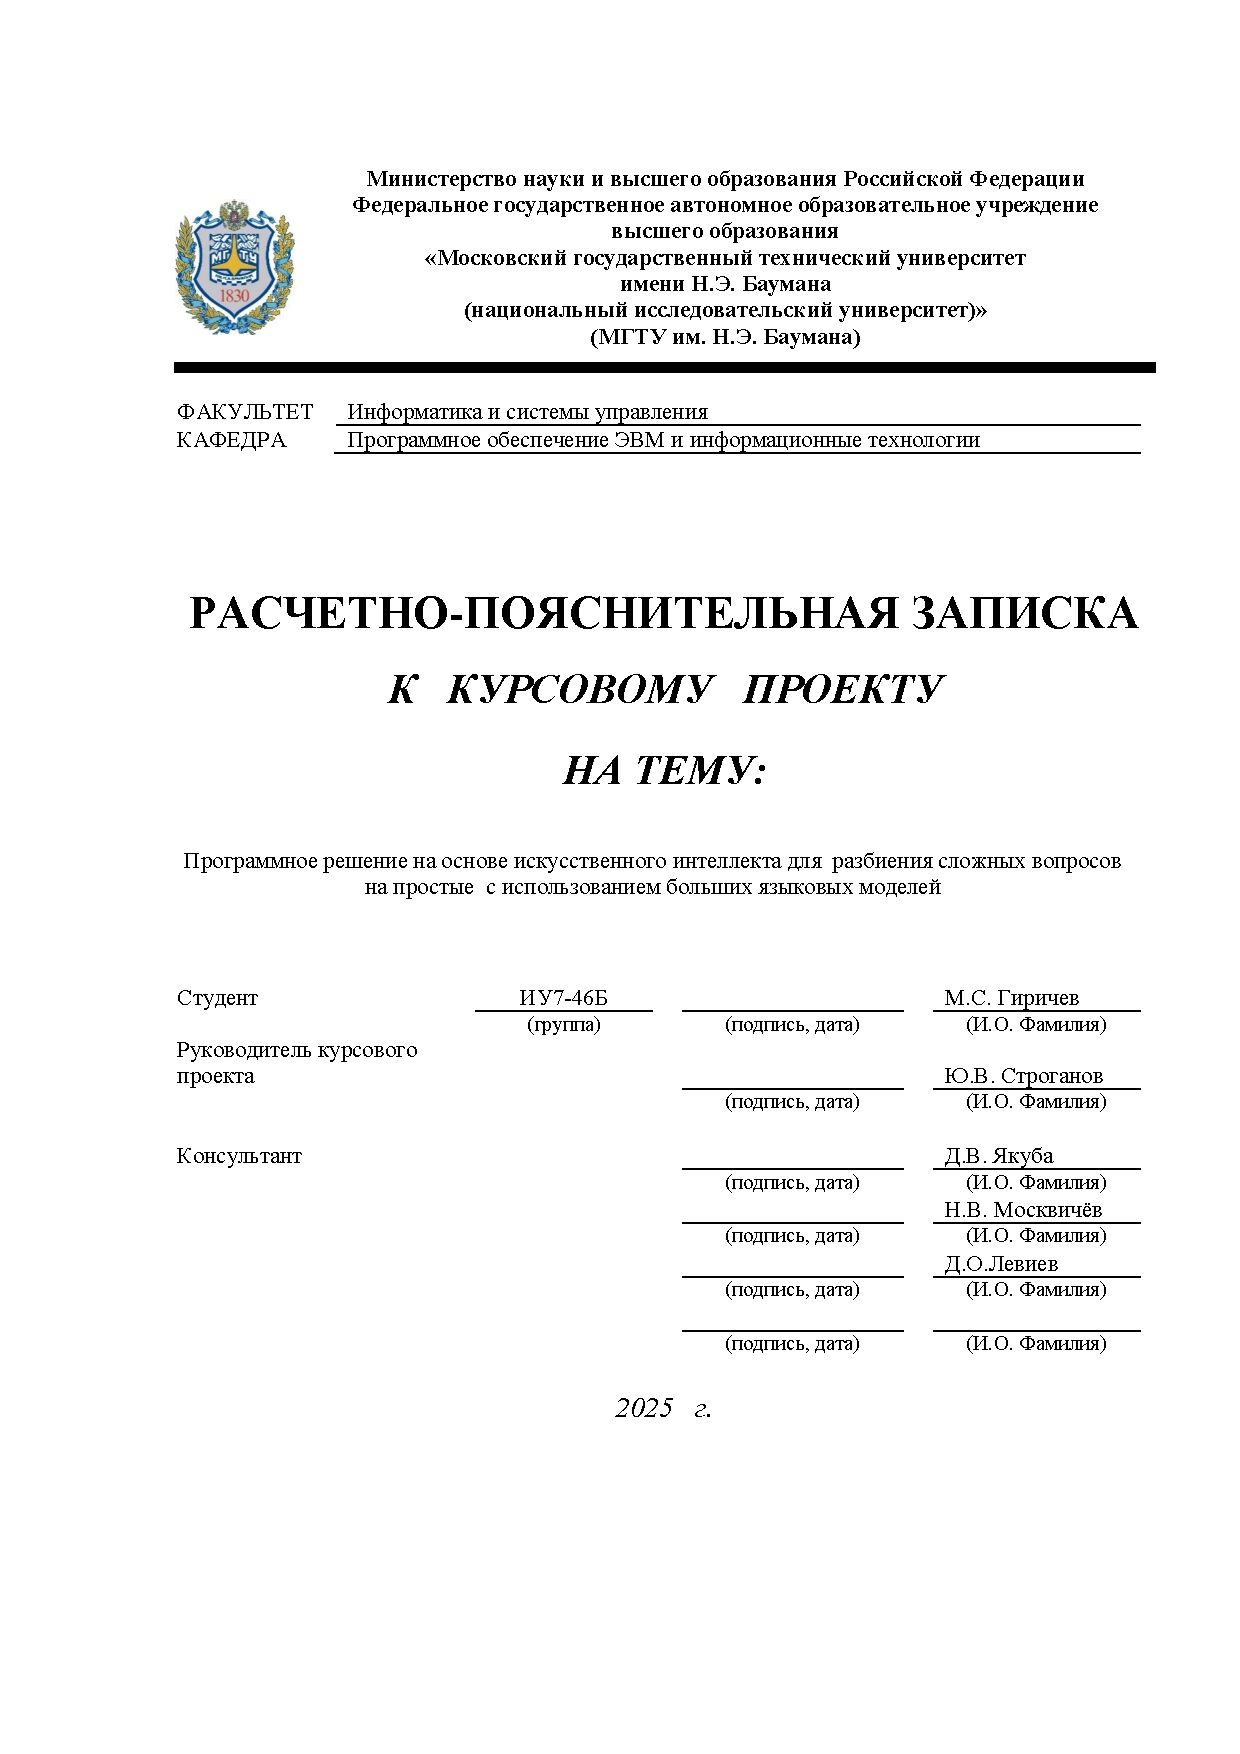
\includepdf[pages=1]{titul.pdf}
	
	\setcounter{page}{4}
	
	\phantomsection
\part*{РЕФЕРАТ}
\addcontentsline{toc}{chapter}{\textbf{РЕФЕРАТ}}

Расчетно-пояснительная записка \pageref{LastPage} с., \totalfigures\ рис., \totaltables\ табл., \total{citnum} ист., \total{appendix}\ прил.

В работе представлено программное решение на основе искусственного интеллекта для разбиения сложных вопросов на простые с использованием больших языковых моделей.

Ключевые слова: большие языковые модели, декомпозиция вопросов, искусственный интеллект, обработка естественного языка, промпт-инженерия.

Проведен комплексный анализ существующих методов декомпозиции вопросов, включая экспертную оценку, алгоритмические методы и методы на основе больших языковых моделей. Разработана трёхуровневая архитектура программного решения, состоящая из модуля консольного интерфейса, модуля управления запросами и модуля взаимодействия с языковой моделью. Реализованы алгоритмы формирования запроса к языковой модели и обработки ответа с многоуровневой валидацией контента. Выполнено исследование эффективности декомпозиции на тестовой выборке из 10 сложных вопросов с экспертной оценкой полноты, атомарности и корректности результатов для 30 языковых моделей. Установлено, что наилучшими показателями обладают проприетарные модели (DeepSeek-V3-Chat, ChatGPT-4, Claude-3-Opus), а среди локальных решений высокую эффективность демонстрируют T-Tech-T-pro-it-1.0 и RuadaptQwen-32B-Pro\_v1. Разработаны правовые механизмы защиты системы в соответствии с требованиями законодательства РФ.
	
	\phantomsection
	\pdfbookmark[0]{\textbf{СОДЕРЖАНИЕ}}{toc}
	\tableofcontents
	
	\phantomsection
\part*{ОПРЕДЕЛЕНИЯ, ОБОЗНАЧЕНИЯ И\\СОКРАЩЕНИЯ}
\addcontentsline{toc}{chapter}{\textbf{ОПРЕДЕЛЕНИЯ, ОБОЗНАЧЕНИЯ И СОКРАЩЕНИЯ}}
В настоящей расчетно-пояснительной записке применяются следующие термины с соответствующими определениями.

\begin{enumdescript}
	\item[Сложный вопрос] -- вопрос, содержащий нескольк аспектов и требующий многокомпонентного ответа.
	
	\item[Простой вопрос] -- самодостаточный атомарный вопрос, фокусирующийся на одном аспекте с определенным ответом.
	
	\item[Модель] -- упрощённое представление реального объекта, процесса или явления, отражающее его существенные свойства.
	
	\item[Языковая модель] -- алгоритмическая система, обученная на больших массивах текста для понимания и генерации естественного языка.
	
	\item[Декомпозиция] -- разделение целого на составные части.
	
	\item[Промпт] -- текстовая инструкция для языковой модели.
	
	\item[Токен] -- минимальная единица текста, обрабатываемая языковой моделью.
	
	\item[ИИ] -- искусственный интеллект.
	
	\item[LLM] -- Large Language Model (большая языковая модель).
	
	\item[QDMR] -- Question Decomposition Meaning Representation (представление смысла декомпозиции вопроса).
	
	\item[EDG] -- Entity Description Graph (граф описания сущностей).
	
	\item[HSP] -- Hierarchical Semantic Parsing (иерархический семантический парсинг).
	
	\item[IDEF0] -- Integration DEFinition for Function Modeling (методология функционального моделирования).
	
	\item[Dependency-граф] -- граф, отражающий синтаксические связи между словами в предложении.
	
	\item[API] -- Application Programming Interface (программный интерфейс приложения).
	
	\item[MMLU] -- Massive Multitask Language Understanding (массовое многозадачное понимание языка).
	
	\item[MATH] -- Mathematics Dataset (набор математических задач для тестирования языковых моделей).
	
	\item[HumanEval] -- набор тестов для оценки способности модели генерировать код.
	
	\item[HellaSwag] -- набор тестов для оценки здравого смысла и понимания контекста.
	
	\item[GPQA] -- General Purpose Question Answering (тест для оценки способности отвечать на общие вопросы).
	
	\item[Квантование] -- метод оптимизации модели путем уменьшения точности представления весов.
	
	\item[Дистилляция] -- процесс передачи знаний от большой модели к меньшей.
	
	\item[Токенизация] -- процесс разбиения текста на минимальные единицы (токены).
	
	\item[Контекстное окно] -- максимальное количество токенов, которое модель может обработать за один раз.
\end{enumdescript}
	
	\phantomsection
\part*{ВВЕДЕНИЕ}
\addcontentsline{toc}{chapter}{\textbf{ВВЕДЕНИЕ}}

Развитие систем искусственного интеллекта создаёт новые возможности для автоматизации сложных интеллектуальных задач. Одной из таких задач является автоматическое разбиение сложных вопросов на простые составляющие. Это особенно актуально в контексте развития больших языковых моделей, которые показывают высокую эффективность при работе с простыми запросами, но часто затрудняются при обработке сложных (комплексных) вопросов. \cite{press2023measuring}

Существующие подходы к декомпозиции вопросов включают как классические методы на основе лингвистического анализа, так и современные решения с использованием нейронных сетей и больших языковых моделей. При этом классические методы часто ограничены жёсткими правилами и шаблонами, в то время как методы на основе ИИ способны адаптироваться к различным формулировкам и контекстам.

Цель работы состоит в разработке программного решения для автоматического разбиения сложных вопросов на простые с использованием больших языковых моделей.

Для достижения поставленной цели определены следующие задачи:

\begin{enumdescript}
	\item анализ существующих методов декомпозиции вопросов;
	\item разработка алгоритма декомпозиции на основе больших языковых моделей;
	\item реализация программного решения;
	\item исследование эффективности разработанного решения.
\end{enumdescript}
	
	\chapter{Аналитический раздел}

\section{Анализ задачи}

Задача декомпозиции сложных вопросов может быть определена как преобразование исходного вопроса в набор более простых, где каждый простой вопрос направлен на получение части информации, необходимой для полного ответа \cite{perez2020unsupervised}. При этом возникают следующие ключевые проблемы:

\begin{enumerate}
	\item определение границ подвопросов: необходимо корректно выделить независимые смысловые части исходного вопроса;
	\item сохранение контекста: простые вопросы должны сохранять связь с контекстом исходного вопроса;
	\item обеспечение полноты: набор простых вопросов должен покрывать всю информационную потребность исходного вопроса;
	\item устранение избыточности: необходимо избегать повторяющихся или пересекающихся подвопросов \cite{barhaim2020quantitative}.
\end{enumerate}

Особую сложность представляют вопросы, содержащие неявные логические связи, требующие понимания контекста и предметной области. Например, вопрос \enquote{Как повлияла индустриальная революция на развитие городов в Европе?} требует учета множества аспектов: экономических, социальных, технологических и демографических изменений.

\section{Анализ существующих решений}

\subsection{Экспертная оценка}

В области декомпозиции сложных вопросов базовым подходом является привлечение экспертов предметной области. Эксперты, опираясь на свои знания и опыт, способны эффективно разбивать сложные вопросы на простые составляющие, учитывая специфику области и контекст. Такой подход обеспечивает высокое качество декомпозиции и позволяет выявлять неочевидные связи между компонентами вопроса, однако имеет ограничения по масштабируемости и требует значительных временных и человеческих ресурсов. \cite{wang2022human}

\subsection{Алгоритмические методы}

\textbf{EDG-Based Question Decomposition} представляет собой комплексный подход к разбиению сложных вопросов, основанный на построении графа описания сущностей (Entity Description Graph). Алгоритм создаёт направленный ациклический граф, где узлы представляют вопросы и сущности, а рёбра отражают логические связи между ними. Особенность метода заключается в использовании итеративного процесса разбиения с применением специализированных правил: W-Rule для обработки вопросительных конструкций, C-Rule для координационных союзов, A-Rule и N-Rule для работы с атрибутивными и именными группами. Эффективность алгоритма подтверждена на задачах построения запросов к базам знаний, однако его производительность существенно зависит от качества начального синтаксического анализа. \cite{hu2021edg}

\textbf{Question Decomposition with Dependency Graphs} реализует подход на основе модели QDMR (Question Decomposition Meaning Representation), где сложный вопрос преобразуется в серию простых вычислительных шагов. Алгоритм применяет конвертацию аннотаций в логические формы и далее в dependency-графы, что позволяет явно моделировать связи между частями вопроса. Метод показывает 16-кратное ускорение по сравнению с другими моделями, однако требует качественной предварительной разметки данных для обучения. \cite{hasson2021question}

\textbf{SPARQA: Skeleton-based Semantic Parsing} предлагает подход к декомпозиции вопросов через построение \enquote{скелета} -- формализации на основе dependency-грамматики. Алгоритм итеративно разбивает вопрос на текстовые span'ы, определяя их взаимосвязи и формируя направленное дерево. Особенность метода заключается в фокусировке на высокоуровневой семантической организации вопроса, что позволяет избежать ошибок dependency-парсинга на длинных сложных конструкциях. Однако метод требует значительных вычислительных ресурсов для построения и анализа скелетной структуры. \cite{sun2020sparqa}

\textbf{Hierarchical Semantic Parsing (HSP)} реализует трёхэтапный подход к декомпозиции вопросов. На первом этапе специальная нейронная модель разбивает исходный вопрос на последовательность подвопросов, затем извлекается ключевая семантическая информация, и наконец происходит интеграция данных для построения логической формы. Метод отличается способностью генерировать полные, естественные подвопросы вместо простого поиска точек разделения, однако требует тщательной настройки параметров для достижения оптимальной производительности. \cite{zhang2019complex}

\subsection{Методы на основе больших языковых моделей}

Большие языковые модели (Large Language Models, LLM) представляют собой особый класс решений для декомпозиции сложных вопросов, не требующий предварительной разработки правил или алгоритмов. В отличие от традиционных подходов, языковые модели способны выполнять декомпозицию, основываясь только на текстовой инструкции (промпте) и собственном обучении на больших массивах текстовых данных. \cite{venktesh2023context} Данный подход значительно упрощает процесс внедрения и масштабирования решений для задач декомпозиции вопросов на практике.

\textbf{DeepSeek} (DeepSeek-V3-Chat) использует архитектуру смеси экспертов, что обеспечивает эффективное распределение вычислительных ресурсов при обработке запросов. Модель демонстрирует высокие результаты в задачах рассуждения и решения проблем, особенно в технических областях, где требуется понимание контекста и многоступенчатый анализ. \cite{deepseek}

\textbf{ChatGPT-4} (chatgpt-4o-latest) представляет собой мультимодальную модель от OpenAI, способную эффективно обрабатывать текст, изображения и аудио данные. Благодаря улучшенной архитектуре и оптимизированным механизмам обработки информации, модель показывает высокую производительность при сниженной стоимости использования по сравнению с предыдущими версиями, что делает её подходящей для широкого спектра приложений. \cite{gpt4}

\textbf{O1} (o1-mini) от OpenAI представляет собой компактную модель, оптимизированную для быстрого отклика и низких вычислительных затрат. Модель использует технологии квантования и дистилляции для достижения баланса между производительностью и качеством, что делает её эффективной для встраиваемых систем и мобильных приложений, где критична скорость работы и ограничены вычислительные ресурсы. \cite{o1}

\textbf{Yi-Lightning} (yi-lightning) использует архитектуру смеси экспертов с оптимизированной системой маршрутизации вычислений. Модель показывает высокие результаты в обработке китайского языка, математических вычислениях и задачах программирования, при этом обеспечивая эффективное использование вычислительных ресурсов. \cite{yi}

\textbf{Claude-3} (claude-3-opus-20240229) от Anthropic реализует комплексный подход к обработке текста и изображений. Модель демонстрирует высокие результаты в тестах MMLU и GPQA, что подтверждает её способность к качественному анализу и обработке сложных запросов в различных предметных областях. \cite{claude}

\textbf{T-Tech} (T-Tech-T-pro-it-1.0) ориентирована на промышленные приложения и обработку технической документации. Модель обучена на корпусе русского и английского языков, что позволяет ей эффективно работать с технической документацией и специализированными текстами в обоих языках. \cite{ttech}

\textbf{GigaChat} (SberDevices-GigaChatMax) представляет собой российскую разработку с расширенными возможностями обработки естественного языка. Модель эффективно справляется с задачами коммуникации на русском языке, генерацией программного кода и аналитической обработкой данных, что делает её востребованной в различных бизнес-приложениях. \cite{gigachat}

\textbf{Gemini} (gemini-1.5-pro-002) от Google обеспечивает комплексную обработку текста, кода и мультимодальных данных. Модель отличается улучшенной производительностью в тестах MMLU и MATH, а оптимизированная система обработки данных позволяет снизить затраты на использование при сохранении высокого качества результатов. \cite{gemini}

\textbf{Qwen} (Qwen2.5-72B-Instruct) от Alibaba поддерживает работу с 29 языками и обеспечивает высокое качество обработки естественного языка. Модель показывает стабильные результаты в задачах программирования и математических вычислениях, что делает её универсальным инструментом для различных прикладных задач. \cite{qwen}

\textbf{Phi} (Phi-4) от Microsoft представляет собой компактную модель с 14 миллиардами параметров. Благодаря специализированной подготовке на качественных наборах данных, модель демонстрирует высокую эффективность в решении математических задач и обработке научных текстов. \cite{phi}

\textbf{LLaMA 3} (llama-3.1-70b-instruct) от Meta обеспечивает высокую производительность в различных задачах обработки естественного языка. Модель успешно проходит тесты HumanEval и MMLU, что подтверждает её способность к анализу и генерации текста в различных предметных областях. \cite{llama}

\textbf{Mistral} (mistral-large-2407) реализует поддержку множества языков программирования и естественных языков. Модель обладает развитыми механизмами рассуждения и доступна через API на различных платформах, что упрощает её интеграцию в существующие системы. \cite{mistral}

\textbf{Command-R+} (command-r-plus) от Cohere разработана для решения корпоративных задач и поддерживает работу с десятью языками. Модель обеспечивает высокую пропускную способность и низкую задержку, что делает её эффективным инструментом для промышленного применения. \cite{cohere}

\textbf{Gemma-2} (gemma-2-9b-it) от Google представляет собой открытую модель, оптимизированную для практического применения. Модель показывает высокие результаты в тестах MMLU и адаптирована для работы как в облачной среде, так и на мобильных устройствах. \cite{gemma}

\textbf{Watari} (Watari-7b-v1) специализируется на обработке японского и английского языков с особым вниманием к языковым нюансам. Модель эффективно обрабатывает различные уровни вежливости в японском языке и поддерживает точный перевод между языками. \cite{watari}

\textbf{YandexGPT} (yandexgpt-4-pro) фокусируется на обработке русского языка и применяется в различных бизнес-задачах. Модель успешно используется для создания контента и разработки чат-ботов, демонстрируя высокую эффективность в задачах на русском языке. \cite{yandexgpt}

\textbf{GPT-3.5 Turbo} (gpt-3.5-turbo-0125) обеспечивает эффективную обработку текста при оптимальном соотношении цены и качества. Модель демонстрирует высокие результаты в тестах HellaSwag и MMLU, что подтверждает её способность к качественному анализу текста в различных контекстах. \cite{gpt35}

\textbf{GLM-4} (glm-4-9b-chat) поддерживает работу с 26 языками и обладает расширенным контекстным окном. Модель включает функционал веб-поиска и выполнения программного кода, что расширяет её возможности в решении практических задач. \cite{chatglm}

\textbf{C4AI Command-R} (c4ai-command-r-v01) оптимизирована для задач рассуждения и обработки текстов. Модель поддерживает работу с большими объемами контекста и включает механизмы проверки генерируемого содержания, что повышает надежность её использования. \cite{c4ai}

\textbf{Suzume} (suzume-llama-3-8b-multilingual) основана на архитектуре LLaMA-3 и адаптирована для многоязычного применения. Модель обучена на большом корпусе диалогов на разных языках, что обеспечивает высокое качество обработки естественного языка в многоязычных приложениях. \cite{suzume}

\textbf{Hermes-2} (hermes-2-theta-llama-3-8b) от Nous Research фокусируется на качественной обработке длительных диалогов. Модель эффективно сохраняет контекст беседы и поддерживает расширенные возможности взаимодействия с пользователем через программные интерфейсы. \cite{hermes}

\textbf{Saiga} (saiga\_llama3\_8b\_v6) разработана для работы с научной литературой в области точных наук. Модель обеспечивает точную обработку математических формул и поддерживает форматирование в LaTeX, что делает её полезным инструментом для научной работы. \cite{saiga}

\textbf{Aya-23-8b} (aya-23-8b) реализует поддержку 23 языков через систему специализированных адаптеров. Модель обеспечивает высокое качество обработки текста для каждого поддерживаемого языка, приближаясь по эффективности к специализированным одноязычным решениям. \cite{aya}

\textbf{Paralex} (paralex-llama-3-8b-sft) ориентирована на обработку юридической и финансовой документации. Модель обеспечивает высокую точность анализа документов и значительно ускоряет процессы их обработки по сравнению с универсальными решениями. \cite{paralex}

\textbf{Storm} (storm-7b) оптимизирована для работы в режиме реального времени на стандартном оборудовании. Модель сохраняет высокий уровень производительности при сниженных требованиях к вычислительным ресурсам, что делает её подходящей для широкого спектра применений. \cite{storm}

\textbf{Neural-Chat} (neural-chat-7b-v3-3) от Intel использует оптимизированные методы вычислений для повышения производительности. Модель поддерживает специализированные инструкции процессоров Intel и обеспечивает эффективную обработку данных на серверном оборудовании. \cite{neural}

\textbf{Vikhr} (vikhr-nemo-12b-instruct-r-21-09-24) представляет собой открытую модель для работы с русским языком. Модель использует специально адаптированную систему токенизации и постоянно совершенствуется через процесс непрерывного обучения. \cite{vikhr}

\textbf{RuadaptQwen} (RuadaptQwen-32B-Pro\_v1) представляет собой адаптированную для русского языка версию модели Qwen2.5-32B с усовершенствованным токенизатором. Модель демонстрирует значительное повышение скорости генерации русскоязычных текстов при сохранении высокого качества ответов и эффективно решает широкий спектр задач обработки естественного языка. \cite{ruadapt}

\textbf{Zero-Mistral} (ru-Zero-Mistral-Small-24B) основана на Mistral-Small-24B-Instruct-2501 с оптимизацией для русского и английского языков. Модель демонстрирует высокую производительность в задачах диалоговых систем и обеспечивает эффективную обработку запросов с сохранением контекста, что делает её подходящей для создания отзывчивых ассистентов. \cite{zeromistral}

\textbf{Cotype-Nano} (MTSAIR-Cotype-Nano) представляет собой легковесную модель, оптимизированную для работы в условиях ограниченных вычислительных ресурсов. Модель разработана с использованием двухэтапного обучения, где MLP-слои тренировались на математических задачах и программном коде, что обеспечивает эффективную обработку запросов на русском и английском языках при сохранении быстродействия. \cite{cotype}

\section{Сравнение больших языковых моделей}

Для объективной оценки возможностей языковых моделей была использована платформа LLM Arena -- открытая краудсорсинговая система оценки больших языковых моделей на русском языке. Платформа использует модель Брэдли-Терри для ранжирования моделей на основе парных сравнений, выполненных людьми, и представляет результаты по шкале Эло. Модель Брэдли-Терри позволяет трансформировать субъективные оценки экспертов в количественные показатели, где вероятность предпочтения одной модели над другой зависит от разницы их рейтингов.

В таблице \ref{tab:llm-comparison} представлены результаты тестирования лучших представителей каждого семейства моделей в категории Arena-Hard-Auto. Для каждой архитектуры или линейки моделей была отобрана версия с наивысшим показателем эффективности, что позволяет провести объективное сравнение различных подходов к построению языковых моделей. Представленные метрики включают: Score -- общий балл модели по шкале Эло, отражающий её относительную силу в сравнении с другими моделями; CI (Confidence Interval) -- доверительный интервал, указывающий на статистическую погрешность оценки; Avg Tokens -- среднее количество токенов в ответе, характеризующее детальность генерируемых текстов; SD (Standard Deviation) -- стандартное отклонение количества токенов, отражающее стабильность объёма ответов; LC (Language Competency) -- оценка языковой компетенции, представляющая собой нормализованный показатель способности модели работать с естественным языком. Высокие значения Score и LC обычно коррелируют с лучшим пользовательским восприятием качества ответов. \cite{llmarena}

\begin{table}[H]
	\caption{Рейтинг языковых моделей по результатам тестирования в LLM Arena}
	\label{tab:llm-comparison}
	\begin{tabular}{|l|c|c|c|c|c|}
		\hline
		\textbf{Модель} & \textbf{Score} & \textbf{CI} & \textbf{Avg Tokens} & \textbf{SD} & \textbf{LC} \\
		\hline
		DeepSeek-V3-Chat & 96.30 & +0.8/-0.7 & 665.97 & 504.83 & 56.62 \\
		chatgpt-4o-latest & 94.74 & +0.8/-1.0 & 693.15 & 634.20 & 56.40 \\
		o1-mini & 93.46 & +0.7/-0.8 & 791.18 & 647.74 & 56.22 \\
		yi-lightning & 93.46 & +0.9/-1.0 & 636.68 & 469.74 & 56.22 \\
		RuadaptQwen-32B-Pro\_v1 & 92.18 & +1.2/-1.2 & 563.43 & 387.83 & 56.04 \\
		claude-3-opus-20240229 & 91.31 & +1.0/-1.1 & 468.69 & 254.10 & 55.92 \\
		T-Tech-T-pro-it-1.0 & 90.87 & +0.8/-1.1 & 502.00 & 380.68 & 55.85 \\
		SberDevices-GigaChatMax & 89.96 & +1.2/-1.4 & 523.95 & 421.87 & 55.73 \\
		gemini-1.5-pro-002 & 89.07 & +1.3/-0.9 & 639.51 & 493.30 & 55.60 \\
		Qwen2.5-72B-Instruct & 88.25 & +0.8/-1.5 & 557.41 & 437.32 & 55.48 \\
		ru-Zero-Mistral-Small-24B & 87.43 & +1.4/-1.2 & 565.19 & 339.27 & 55.37 \\
		vikhr-nemo-12b-instruct-r & 87.31 & +1.1/-1.4 & 627.00 & 416.72 & 55.35 \\
		Phi-4 & 86.59 & +1.1/-1.3 & 641.70 & 439.80 & 55.25 \\
		llama-3.1-70b-instruct & 83.26 & +1.4/-1.1 & 537.53 & 428.60 & 54.77 \\
		mistral-large-2407 & 80.40 & +2.1/-1.5 & 422.42 & 320.72 & 54.36 \\
		command-r-plus & 77.17 & +1.5/-1.5 & 560.83 & 424.07 & 53.90 \\
		gemma-2-9b-it & 76.50 & +1.3/-1.3 & 459.15 & 312.59 & 53.81 \\
		Watari-7b-v1 & 69.49 & +1.7/-1.7 & 616.80 & 449.25 & 52.80 \\
		yandexgpt-4-pro & 59.24 & +2.1/-1.9 & 383.80 & 306.97 & 51.33 \\
		MTSAIR-Cotype-Nano & 50.51 & +1.9 / -1.4 & 567.34 & 435.47 & 50.07 \\
		gpt-3.5-turbo-0125 & 50.00 & +0.0/-0.0 & 220.83 & 170.30 & 50.00 \\
		glm-4-9b-chat & 49.75 & +2.0/-2.0 & 568.81 & 448.76 & 49.96 \\
		c4ai-command-r-v01 & 48.95 & +3.0/-2.1 & 529.34 & 368.98 & 49.85 \\
		suzume-llama-3-8b & 45.71 & +2.3/-2.6 & 641.18 & 858.96 & 49.38 \\
		hermes-2-theta-llama-3-8b & 44.08 & +2.4/-2.3 & 485.99 & 390.85 & 49.15 \\
		saiga\_llama3\_8b\_v6 & 39.17 & +2.1/-1.6 & 471.51 & 463.62 & 48.44 \\
		aya-23-8b & 36.26 & +1.9/-2.2 & 554.34 & 433.51 & 48.02 \\
		paralex-llama-3-8b-sft & 37.36 & +2.5/-2.2 & 688.57 & 632.87 & 48.18 \\
		storm-7b & 20.62 & +1.7/-1.4 & 419.32 & 190.85 & 45.78 \\
		neural-chat-7b-v3-3 & 19.04 & +1.5/-1.5 & 927.21 & 1211.62 & 45.56 \\
		\hline
	\end{tabular}
\end{table}

\section{Модель разрабатываемого процесса}

Для наглядного представления процесса разбиения сложных вопросов на простые была создана IDEF0-диаграмма (рисунок \ref{fig:idef0}). На ней показано, как сложный вопрос преобразуется в набор простых вопросов.

После анализа всех рассмотренных методов, для решения задачи лучше всего подходят большие языковые модели. Это объясняется несколькими причинами:
\begin{itemize}
	\item отсутствие необходимости в разработке сложных правил и алгоритмов;
	\item высокая адаптивность к различным типам вопросов и предметным областям;
	\item возможность сохранения контекста и логических связей между частями вопроса;
	\item простота интеграции и масштабирования решения.
\end{itemize}

\begin{figure}[H]
	\centering
	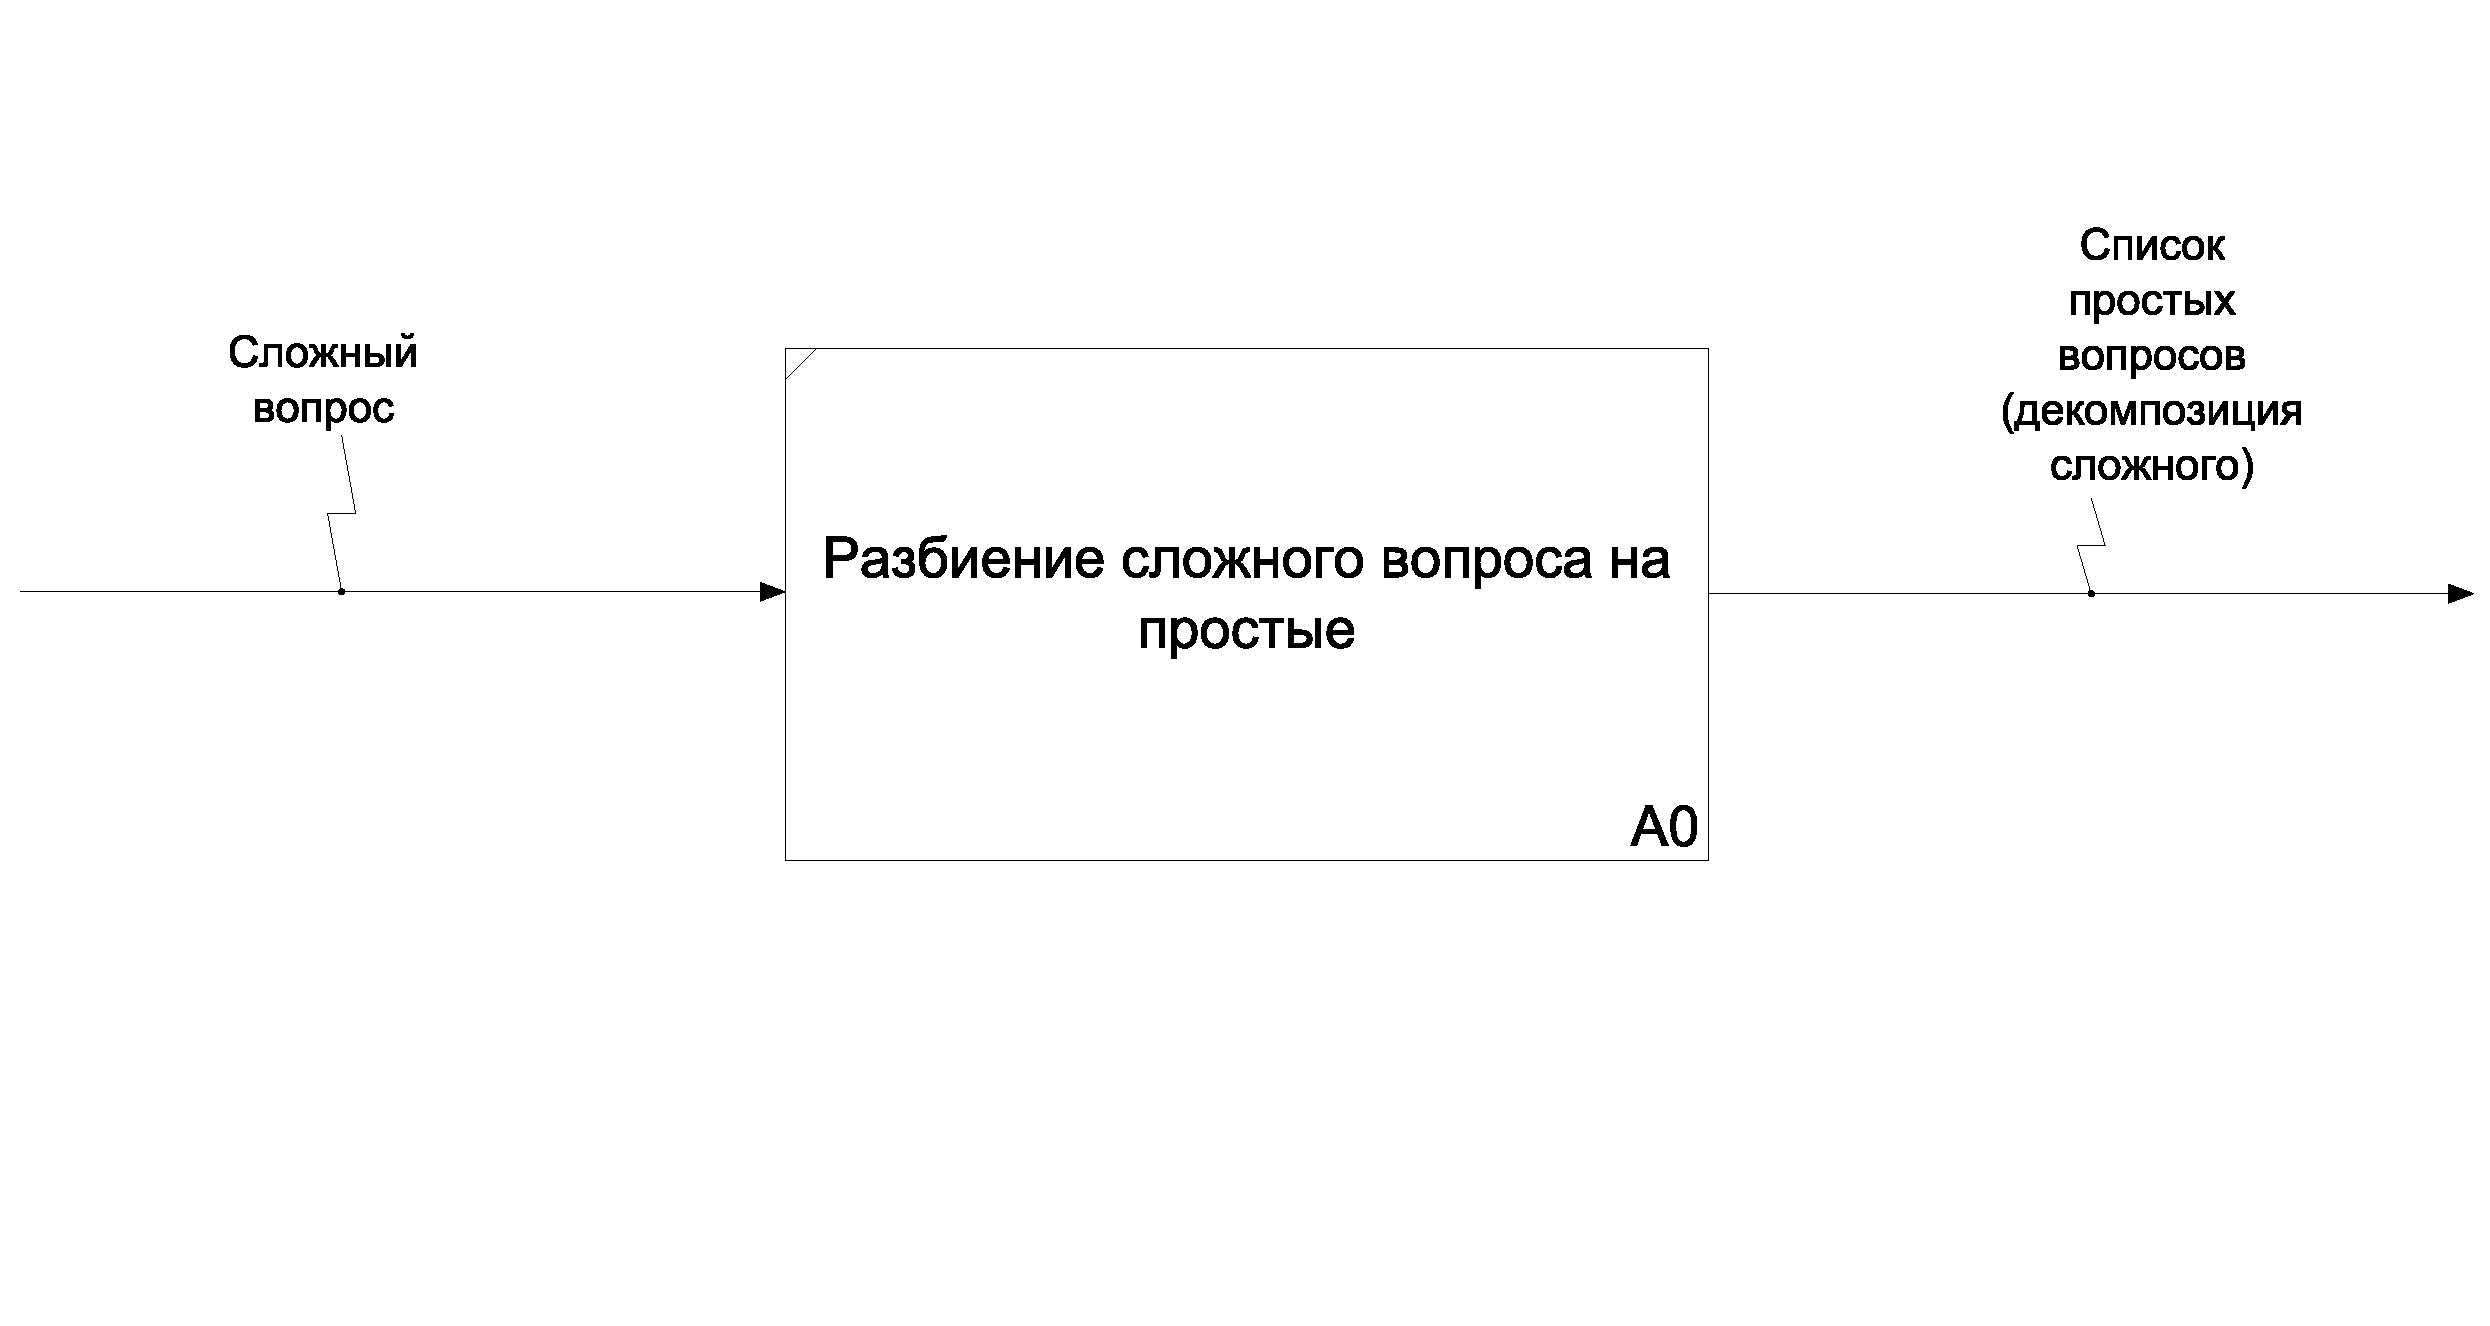
\includegraphics[width=0.8\textwidth]{images/analyth_idef0.pdf}
	\caption{Функциональная модель процесса разбиения сложных вопросов на простые}
	\label{fig:idef0}
\end{figure}

\section{Вывод}

В аналитическом разделе был проведен комплексный анализ задачи разбиения сложных вопросов на простые. Рассмотрены основные проблемы и требования к процессу декомпозиции, исследованы существующие подходы в трёх категориях: экспертная оценка, алгоритмические методы и методы на основе больших языковых моделей. Проанализировано более 30 существующих решений с точки зрения их применимости к решению поставленной задачи.

На основе проведенного анализа разработана функциональная модель процесса, в которой декомпозиция вопроса осуществляется с помощью языковой модели. Такой подход позволяет эффективно решать поставленную задачу, обеспечивая необходимую гибкость и качество результатов при минимальных требованиях к разработке дополнительных компонентов системы.
	
	\chapter{Конструкторский раздел}

\section{Функциональная модель системы}

Функциональная модель системы декомпозиции сложных вопросов представляет процесс преобразования исходного сложного вопроса в набор более простых. Данный процесс реализуется с помощью локальной языковой модели, которая получает специально сформированные инструкции (промпты) для выполнения декомпозиции.

Проектируемая система основана на результатах анализа существующих решений, проведенного в аналитическом разделе. Для реализации выбран подход с использованием локальной языковой модели, что позволяет обеспечить высокую адаптивность к различным типам вопросов при сохранении контекста и логических связей, а также независимость от внешних сервисов.

Для формализации процесса декомпозиции разработана функциональная модель в нотации IDEF0, представленная на диаграммах нулевого и первого уровней (рисунки \ref{fig:constr_idef0_level0}, \ref{fig:constr_idef0_level1}).

\begin{figure}[h]
	\centering
	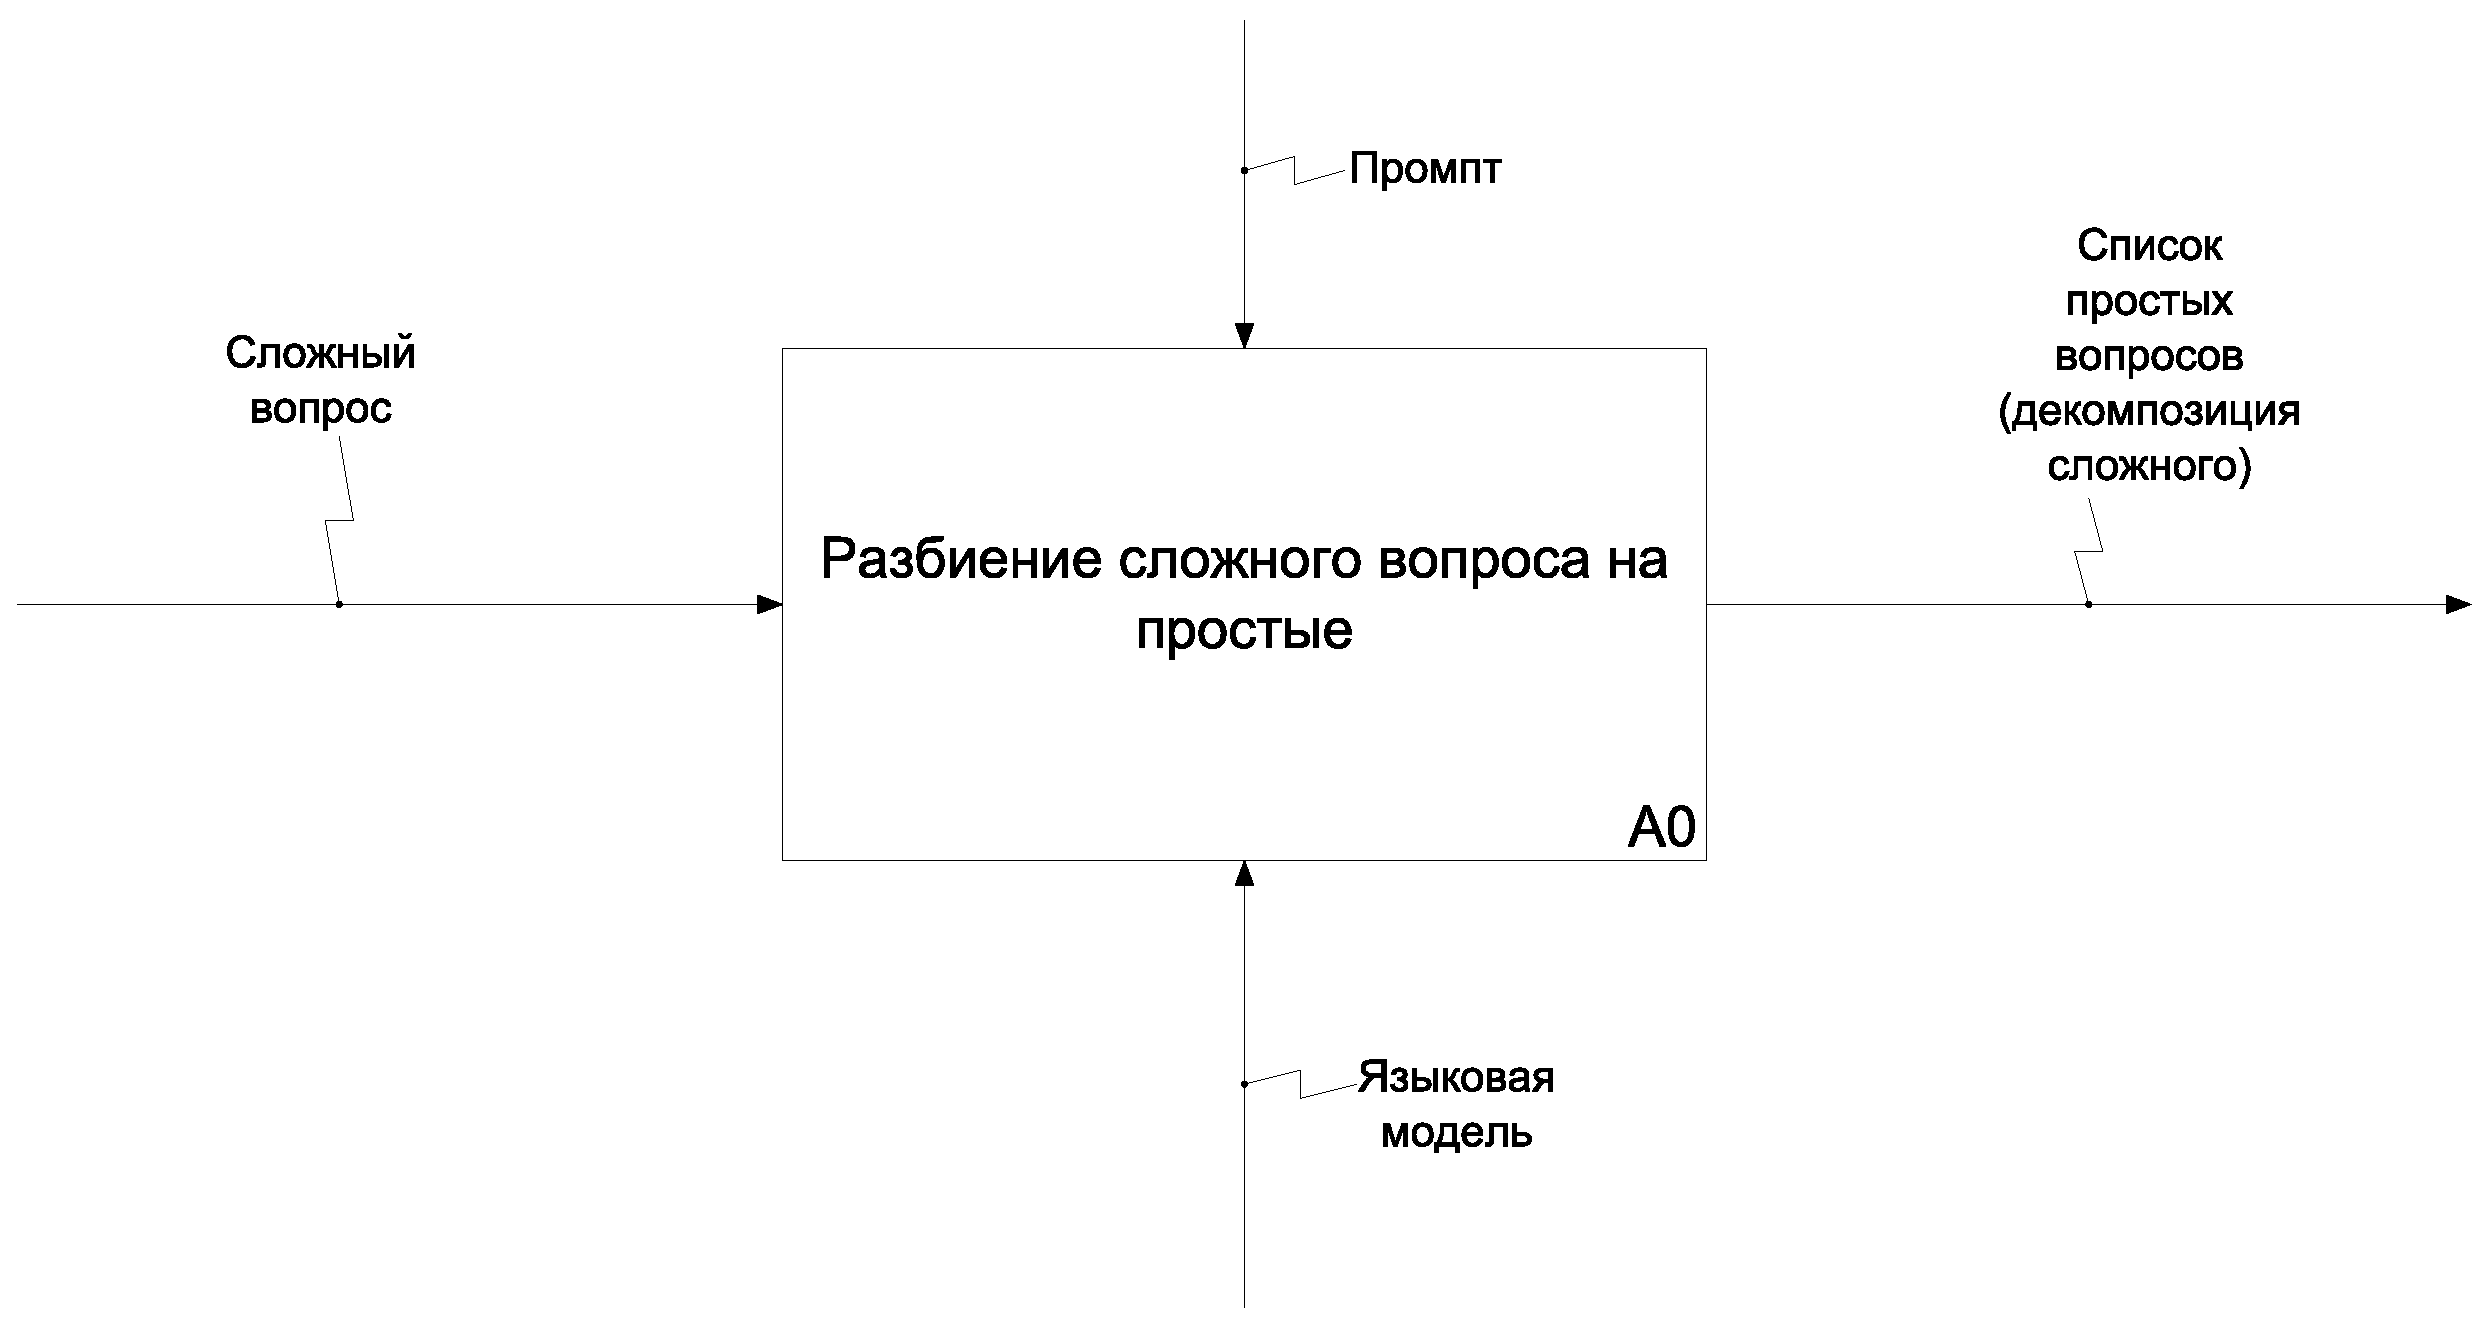
\includegraphics[width=0.8\textwidth]{images/idef0_level0.pdf}
	\caption{Функциональная модель процесса разбиения сложных вопросов (нулевой уровень)}
	\label{fig:constr_idef0_level0}
\end{figure}

\newpage

Для более детального представления структуры системы разработана модель первого уровня, которая включает три последовательных процесса:
\begin{enumerate}
	\item формирование запроса к языковой модели;
	\item взаимодействие с языковой моделью;
	\item формирование результата декомпозиции.
\end{enumerate}

\begin{figure}[h]
	\centering
	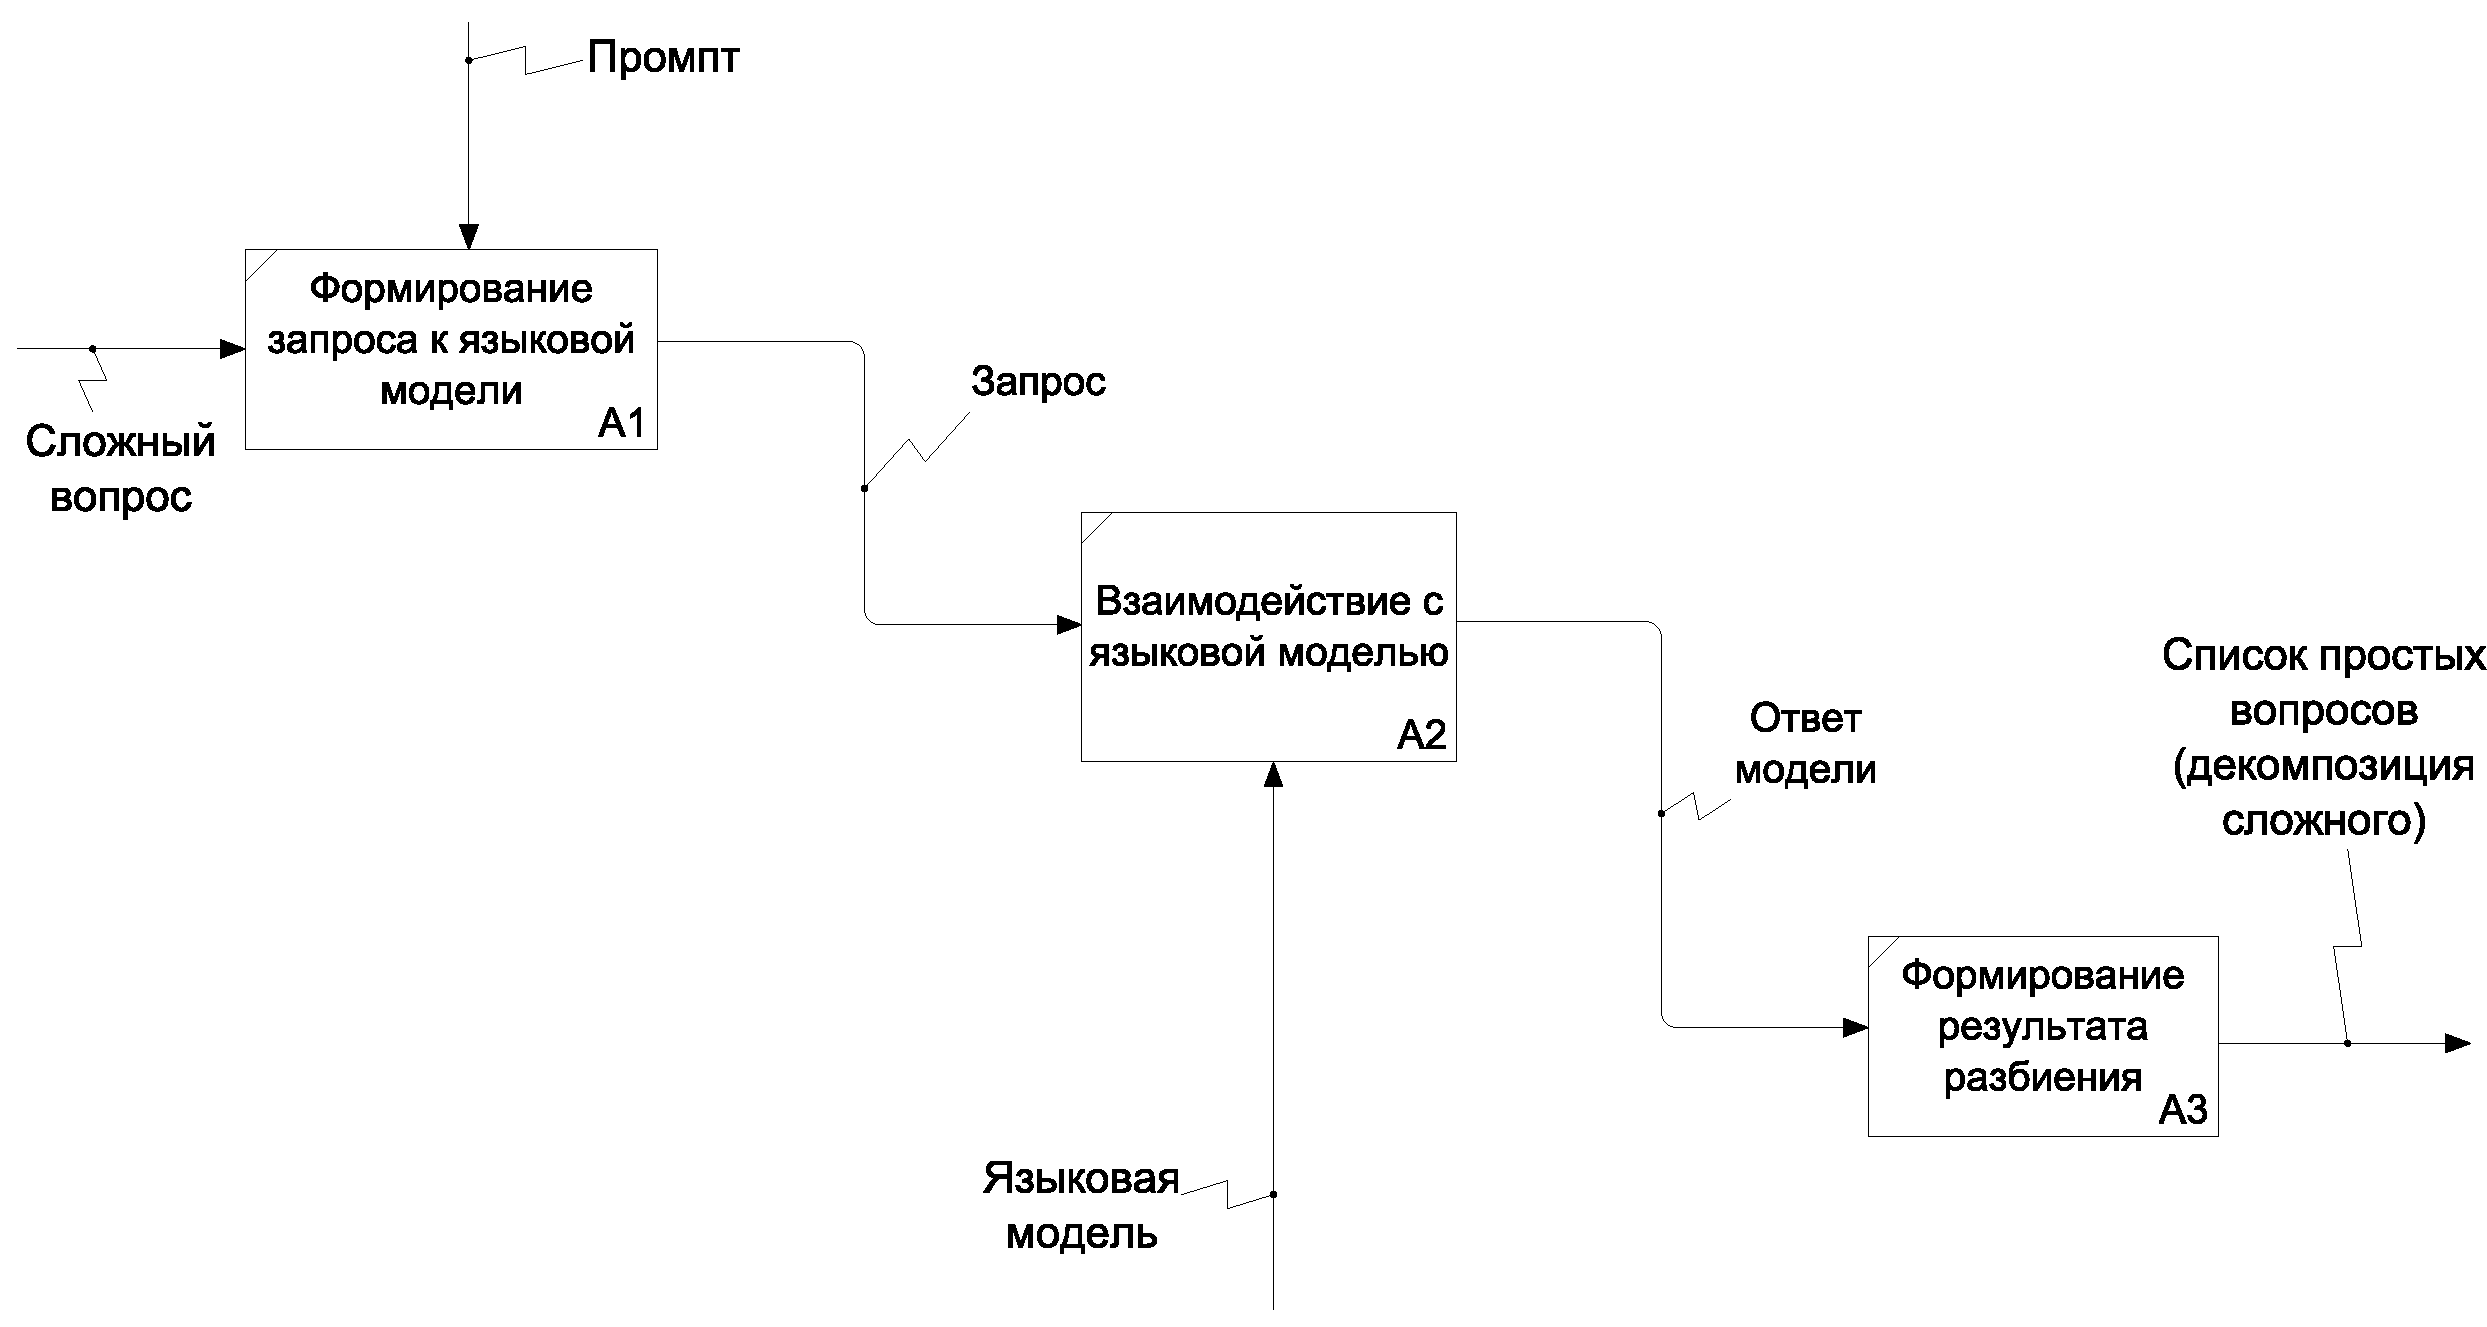
\includegraphics[width=0.8\textwidth]{images/idef0_level1.pdf}
	\caption{Функциональная модель процесса разбиения сложных вопросов (первый уровень)}
	\label{fig:constr_idef0_level1}
\end{figure}

Декомпозиция процесса позволяет выделить три ключевых этапа обработки вопроса. На первом этапе исходный сложный вопрос преобразуется в формат запроса для языковой модели с добавлением промпта. Далее подготовленный запрос передается в языковую модель, которая генерирует ответ согласно полученным инструкциям. На заключительном этапе система обрабатывает полученный от модели ответ, структурирует его и формирует итоговый список простых вопросов.

Разделение на отдельные процессы позволяет локализовать компоненты системы и обеспечить их независимую модификацию и тестирование. Такой подход также упрощает интеграцию различных языковых моделей и форматов представления данных.

\section{Архитектура программного решения}

Программное решение для декомпозиции сложных вопросов построено на модульном принципе, что обеспечивает гибкость системы и возможность ее адаптации к различным требованиям. Архитектура включает три основных модуля, взаимодействующих между собой для обеспечения полного цикла обработки вопросов (рисунок \ref{fig:constr_architecture}).

\begin{figure}[H]
	\centering
	\begin{tikzpicture}[
		box/.style={draw, rectangle, minimum width=6cm, minimum height=1.8cm, thick},
		arrow/.style={->, >=latex, thick},
		node distance=3.5cm
		]
		
		% Модули - располагаем вертикально
		\node[box] (ui) at (0,0) {Модуль консольного интерфейса};
		\node[box] (manager) at (0,-4) {Модуль управления запросами};
		\node[box] (model) at (0,-8) {Модуль взаимодействия с языковой моделью};
		
		% Стрелки вниз по левой части
		\draw[arrow] ([xshift=-1cm]ui.south) -- node[left] {Вопрос} ([xshift=-1cm]manager.north);
		\draw[arrow] ([xshift=-1cm]manager.south) -- node[left] {Запрос} ([xshift=-1cm]model.north);
		
		% Стрелки вверх по правой части
		\draw[arrow] ([xshift=1cm]model.north) -- node[right] {Ответ} ([xshift=1cm]manager.south);
		\draw[arrow] ([xshift=1cm]manager.north) -- node[right] {Результат} ([xshift=1cm]ui.south);
		
	\end{tikzpicture}
	\caption{Архитектура программного решения}
	\label{fig:constr_architecture}
\end{figure}

Основные модули системы и их функции:

\begin{enumerate}
	\item Модуль консольного интерфейса отвечает за взаимодействие с пользователем через командную строку. Основные функции модуля включают чтение сложных вопросов из указанных пользователем текстовых файлов и запись результатов декомпозиции в выходные файлы. Модуль поддерживает базовые команды для управления процессом и настройками приложения.

	\item Модуль управления запросами осуществляет подготовку запроса к языковой модели с добавлением необходимых инструкций и обработку полученных результатов. Данный модуль также выполняет фильтрацию входных запросов и выходных ответов на предмет наличия запрещенных слов по предустановленному списку. Модуль связывает интерфейс пользователя с языковой моделью и обеспечивает корректную передачу данных между ними.

	\item Модуль взаимодействия с языковой моделью обеспечивает коммуникацию с локальной языковой моделью, передачу запросов и получение ответов. Модуль содержит механизмы обработки ошибок для обеспечения надежности системы.
\end{enumerate}

Взаимодействие между модулями построено по принципу последовательной обработки данных. Модуль консольного интерфейса считывает вопрос из указанного пользователем файла и передает его в модуль управления запросами. Этот модуль формирует полный запрос и передает его в модуль взаимодействия с языковой моделью. После получения ответа от модели данные проходят обратный путь: модуль взаимодействия передает их в модуль управления запросами для структурирования, после чего результат передается в модуль консольного интерфейса для записи в выходной файл.

\section{Алгоритмическое обеспечение}



\subsection{Алгоритм формирования запроса к языковой модели}

Алгоритм формирования запроса предназначен для подготовки структурированного запроса к языковой модели, включающего оригинальный вопрос пользователя и специализированный промпт с инструкциями по декомпозиции (рисунок \ref{fig:constr_prompt_algorithm}). Он представляет собой последовательность действий от получения исходного вопроса до формирования полного запроса к модели. 

Алгоритм включает следующие шаги:
\begin{enumerate}
	\item получение исходного вопроса из указанного файла;
	\item загрузка шаблона промпта из конфигурационного файла;
	\item объединение промпта и вопроса пользователя в единый запрос;
	\item проверка запроса на наличие запрещенных слов по предустановленному списку;
	\item форматирование запроса для передачи языковой модели;
	\item возвращение готового запроса для дальнейшей обработки.
\end{enumerate}

Временная сложность алгоритма: $O(n)$, где $n$ -- длина исходного вопроса и промпта.
Требования к памяти: $O(n)$, необходимая память линейно зависит от размера вопроса и промпта.

\begin{figure}[H]
	\centering
	\begin{tikzpicture}[
		start/.style={draw, rounded rectangle, minimum width=4.5cm, minimum height=1cm, thick},
		process/.style={draw, rectangle, minimum width=4.5cm, minimum height=1cm, thick},
		end/.style={draw, rounded rectangle, minimum width=4.5cm, minimum height=1cm, thick},
		arrow/.style={->, >=latex, thick},
		node distance=2cm
		]
		
		% Элементы блок-схемы
		\node[start] (start) {Начало};
		\node[process, below=of start] (input) {Получение вопроса из консоли};
		\node[process, below=of input] (load) {Загрузка шаблона промпта};
		\node[process, below=of load] (combine) {Объединение промпта и вопроса};
		\node[process, below=of combine] (format) {Форматирование запроса};
		\node[end, below=of format] (end) {Конец};
		
		% Стрелки с текстом
		\draw[arrow] (start) -- node[right] {Ввод пользователя} (input);
		\draw[arrow] (input) -- node[right] {Конфигурационный файл} (load);
		\draw[arrow] (load) -- node[right] {Подготовка контекста} (combine);
		\draw[arrow] (combine) -- node[right] {Создание структуры запроса} (format);
		\draw[arrow] (format) -- node[right] {Возврат готового запроса} (end);
		
	\end{tikzpicture}
	\caption{Алгоритм формирования запроса к языковой модели}
	\label{fig:constr_prompt_algorithm}
\end{figure}

\subsection{Алгоритм обработки ответа языковой модели}

Алгоритм обработки ответа предназначен для структурирования результата, полученного от языковой модели, в заданный формат (список вопрос), который ожидает пользователь (рисунок \ref{fig:constr_response_algorithm}).

\begin{figure}[H]
	\centering
	\begin{tikzpicture}[
		start/.style={draw, rounded rectangle, minimum width=4.5cm, minimum height=1cm, thick},
		process/.style={draw, rectangle, minimum width=4.5cm, minimum height=1cm, thick},
		decision/.style={draw, diamond, minimum width=4.5cm, minimum height=2.5cm, aspect=2, thick},
		end/.style={draw, rounded rectangle, minimum width=4.5cm, minimum height=1cm, thick},
		arrow/.style={->, >=latex, thick},
		node distance=2.5cm
		]
		
		% Элементы блок-схемы
		\node[start] (start) {Начало};
		\node[process, below=of start] (receive) {Получение ответа модели};
		\node[decision, below=of receive] (error) {Есть ошибки?};
		\node[process, below=2cm of error, xshift=-4.5cm] (error_handle) {Обработка ошибки};
		\node[process, below=2cm of error, xshift=4.5cm] (parse) {Разбор текста ответа};
		\node[process, below=of parse] (filter) {Фильтрация результатов};
		\node[process, below=of filter] (format) {Форматирование списка};
		\node[end, below=of format] (end) {Конец};
		
		% Стрелки с текстом
		\draw[arrow] (start) -- node[right] {Вопрос от пользователя} (receive);
		\draw[arrow] (receive) -- node[right] {Ответ модели} (error);
		\draw[arrow] (error.west) -- ++(-2.109,0) to[out=-90, in=90] (error_handle.north) node[above, pos=0.5, yshift=2pt] {Да};
		\draw[arrow] (error.east) -- ++(2.109,0) to[out=-90, in=90] (parse.north) node[above, pos=0.5, yshift=2pt] {Нет};
		
		\draw[thick] (error_handle) -- ++(0,-9cm) -| node[left, pos=0.3, yshift=4.8cm] {Сообщение об ошибке} ($(format)!0.5!(end)$);
		\draw[arrow] (parse) -- node[right] {Извлечение вопросов} (filter);
		\draw[arrow] (filter) -- node[right] {Удаление дубликатов} (format);
		\draw[arrow] (format) -- node[right, align=left] {Создание списка \\ простых вопросов} (end);
		
	\end{tikzpicture}
	\caption{Алгоритм обработки ответа языковой модели}
	\label{fig:constr_response_algorithm}
\end{figure}

\newpage

Алгоритм обработки ответа иллюстрирует процесс извлечения и структурирования простых вопросов из текстового ответа языковой модели. Включает проверки на наличие ошибок и корректность формата ответа.

Алгоритм состоит из следующих шагов:
\begin{enumerate}
	\item получение текстового ответа от языковой модели;
	\item проверка на наличие ошибок в ответе модели;
	\item разбор текстового ответа и извлечение отдельных вопросов;
	\item проверка извлеченных вопросов на наличие запрещенных слов;
	\item фильтрация и удаление возможных дубликатов или нерелевантных элементов;
	\item форматирование результата в структурированный список вопросов;
	\item сохранение готового списка простых вопросов в выходной файл.
\end{enumerate}

Временная сложность алгоритма: $O(m)$, где $m$ -- длина ответа языковой модели.
Требования к памяти: $O(m)$, необходимая память линейно зависит от размера ответа.

\section{Сценарий использования системы}

Основной сценарий использования консольного приложения включает:
\begin{enumerate}
	\item запуск приложения через командную строку;
	\item формирование системой запроса к языковой модели;
	\item отправка запроса в локальную языковую модель и получение ответа;
	\item обработка ответа и формирование списка простых вопросов;
	\item запись результата в указанный файл в виде пронумерованного списка простых вопросов.
\end{enumerate}

\section{Требования к консольному интерфейсу}

Консольный интерфейс системы должен обеспечивать:
\begin{itemize}
	\item поддержку пакетного режима обработки нескольких файлов;
	\item поддержку базовых команд: декомпозиция, справка, завершение работы;
	\item отображение процесса обработки запроса (вывод названия текущего процесса);
	\item формирование диагностических сообщений при возникновении ошибок.
\end{itemize}

\section{Процессная модель системы}

Для наглядного представления последовательности операций и взаимодействия между компонентами системы разработана процессная модель декомпозиции сложных вопросов в нотации BPMN (Business Process Model and Notation), представленная на рисунок \ref{fig:constr_bpmn}.

\begin{figure}[H]
	\centering
	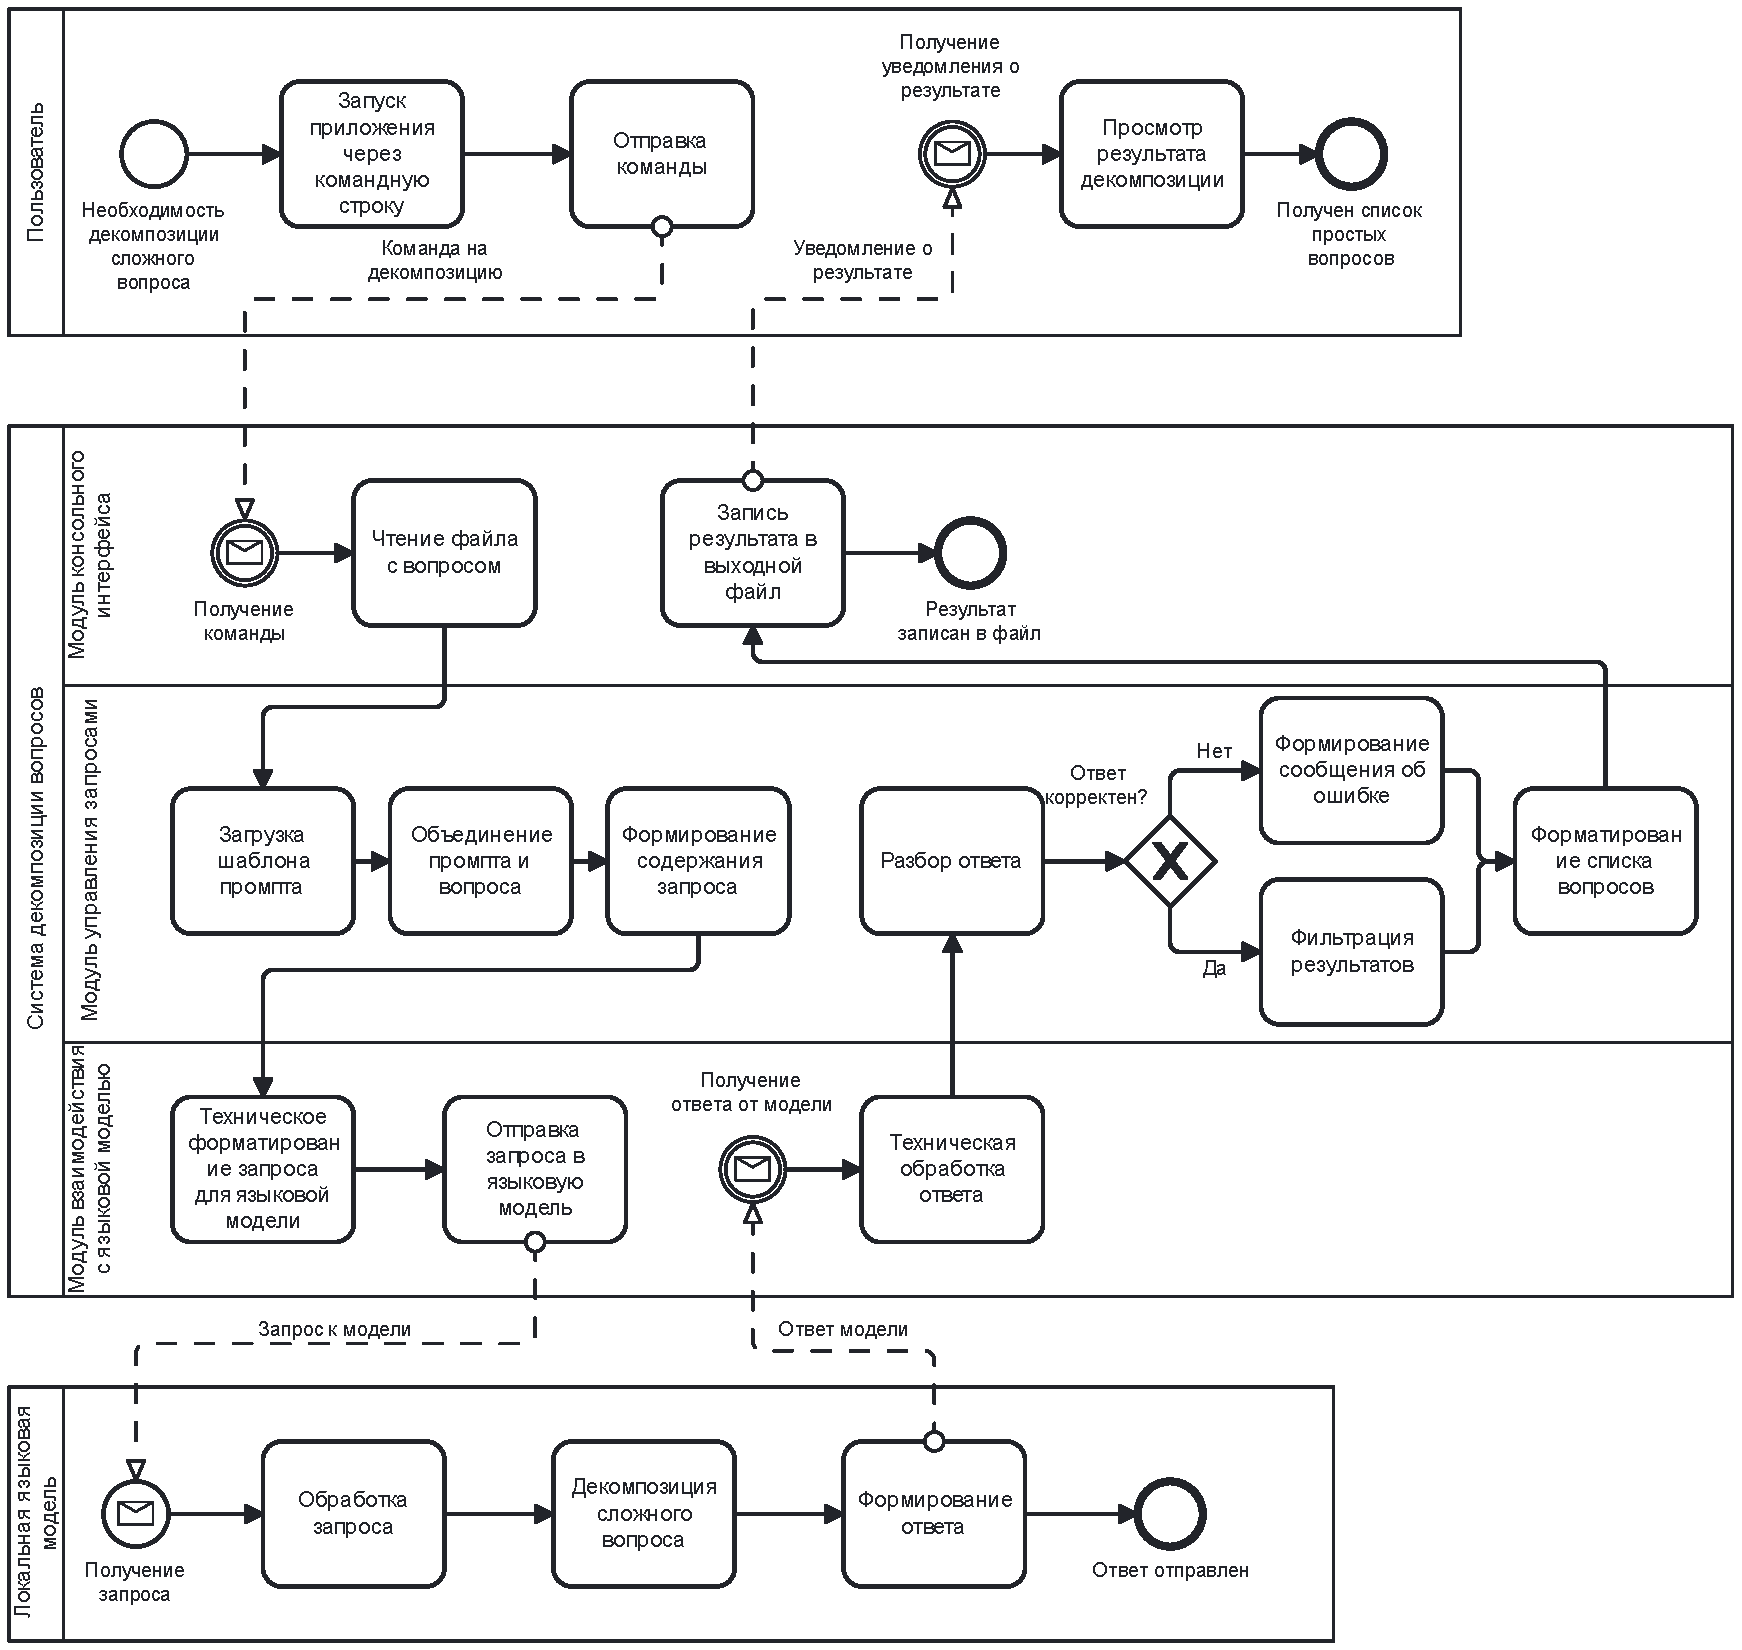
\includegraphics[width=1\textwidth]{images/BPMN.pdf}
	\caption{Процессная модель декомпозиции сложных вопросов в нотации BPMN}
	\label{fig:constr_bpmn}
\end{figure}

Данная модель детализирует взаимодействие четырех основных участников процесса:
\begin{itemize}
	\item пользователь системы, инициирующий декомпозицию вопроса;
	\item модуль консольного интерфейса, обеспечивающий ввод-вывод данных;
	\item система декомпозиции вопросов, включающая модуль управления запросами и модуль взаимодействия с языковой моделью;
	\item локальная языковая модель, выполняющая непосредственную декомпозицию.
\end{itemize}

Представленная процессная модель иллюстрирует полный жизненный цикл декомпозиции вопроса -- от момента запуска приложения пользователем до получения структурированного списка простых вопросов. В модели отражены точки принятия решений, например, проверка корректности ответа модели, которая позволяет обрабатывать нестандартные ситуации.

Модель также демонстрирует распределение задач между тремя основными модулями системы и позволяет визуализировать потоки данных между ними. Такое представление обеспечивает комплексное понимание процесса декомпозиции и возможность анализа системы на предмет оптимизации взаимодействия между компонентами.

\section{Параметры системы}

\subsection{Временные характеристики}

Для обеспечения приемлемого пользовательского опыта система должна соответствовать следующим временным характеристикам:
\begin{itemize}
	\item время формирования запроса к языковой модели: не более 0.01 секунды;
	\item время обработки запроса языковой моделью: не более 60 секунд для сложных вопросов (зависит от размера модели и вычислительных ресурсов);
	\item время обработки ответа и формирования результата: не более 60 секунд (зависит от размера модели и вычислительных ресурсов).
\end{itemize}

\subsection{Параметры языковой модели}

К используемой локальной языковой модели предъявляются следующие требования:
\begin{itemize}
	\item поддержка контекстного окна не менее 2000 токенов для обработки сложных вопросов;
	\item возможность работы с русским языком;
	\item способность следовать инструкциям в промпте для структурированного вывода;
	\item производительность, достаточная для обработки запроса в рамках установленных временных ограничений.
\end{itemize}

\section{Вывод}

В конструкторском разделе разработана функциональная модель системы декомпозиции сложных вопросов на простые с использованием локальной языковой модели. Определена архитектура программного решения, включающая три основных модуля: консольный интерфейс, управление запросами и взаимодействие с языковой моделью.

Предложены алгоритмы формирования запроса к языковой модели и обработки полученных результатов, определены их временные и пространственные характеристики. Описаны основные сценарии использования системы, включая работу с файлами для ввода сложных вопросов и вывода результатов декомпозиции.

Установлены временные характеристики работы системы и требования к используемой языковой модели. Сформулированы системные требования для функционирования программного решения с локальной языковой моделью.

Разработанное проектное решение обеспечивает основу для реализации системы декомпозиции сложных вопросов, отвечающей требованиям надежности и интуитивности использования.
	
	\chapter{Технологический раздел}

\section{Выбор средств разработки}

В данном разделе обосновывается выбор технологий и инструментов, используемых для реализации программного решения декомпозиции сложных вопросов на простые.

\subsection{Язык программирования}

Для реализации программного решения использован язык Python версии 3.11. Выбор обусловлен следующими факторами:

\begin{enumdescript}
	\item наличие готовых библиотек для работы с NLP и языковыми моделями;
	\item относительная простота синтаксиса, что сокращает время разработки;
	\item поддержка основных операционных систем (Windows, Linux, macOS);
	\item простота интеграции с локальными моделями машинного обучения через существующие Python-обертки;
	\item возможность применять как объектно-ориентированный, так и функциональный подходы при необходимости.
\end{enumdescript}

\subsection{Библиотеки и фреймворки}

Для реализации программного решения использованы следующие библиотеки:

\begin{enumdescript}
	\item \textbf{llama-cpp-python} \cite{llama_cpp_lib}:
	\begin{itemize}
		\item python-обертка для llama.cpp, позволяющая запускать локальные языковые модели;
		\item запуск выполнение моделей на CPU и опционально на GPU;
		\item поддержка различных форматов моделей (GGUF, GGML);
	\end{itemize}
	
	\item \textbf{typer} \cite{typer_lib}:
	\begin{itemize}
		\item создание CLI-приложений с типизированными аргументами;
		\item автоматическая валидация входных данных;
		\item генерация справочной документации;
		\item поддержка подкоманд и расширенная обработка ошибок.
	\end{itemize}
	
	\item \textbf{rich} \cite{rich_lib}:
	\begin{itemize}
		\item форматированный вывод в терминале с поддержкой цветов и стилей;
		\item отображение прогресса выполнения операций;
	\end{itemize}
	
	\item \textbf{pydantic} \cite{pydantic_lib}:
	\begin{itemize}
		\item валидация данных и управление настройками приложения;
		\item автоматическая сериализация/десериализация данных;
		\item поддержка схем валидации на основе аннотаций типов python.
	\end{itemize}
\end{enumdescript}

\subsection{Среда разработки}

Разработка программного решения велась в операционной системе \textbf{Windows 11}. В качестве интегрированной среды разработки использовался \textbf{Visual Studio Code}.

\section{Модульная структура программного решения}

Разработанное решение представляет собой консольное приложение, структура которого соответствует архитектуре, спроектированной в конструкторском разделе. Программа состоит из трех основных модулей, каждый из которых выполняет определенную функцию в процессе декомпозиции вопросов.

Структура файлов проекта организована следующим образом:
\begin{lstlisting}[caption={Файловая структура проекта}, label=lst:project_struct, language=Python]
 project/
 ├───configs/
 │    └──config.json           # Конфигурационный файл
 │       
 ├───examples/                 # Примеры входных данных
 │    ├──question1.txt
 │    └──question2.txt
 │       
 ├───models/                   # Директория для файлов языковых моделей
 │    └──t-lite-it-1.0-q4_k_m.gguf
 │       
 ├───results/                  # Результаты работы программы
 │    ├──answers1.txt
 │    └──answers2.txt
 │       
 └───src/                      # Исходный код программы
	  ├──cli_module.py         # Модуль консольного интерфейса
 	  ├──model_module.py       # Модуль взаимодействия с языковой моделью
 	  ├──request_module.py     # Модуль управления запросами
 	  ├──curse_words.txt       # Список запрещённых слов
 	  └──__init__.py
\end{lstlisting}

\subsection{Модуль консольного интерфейса}

Модуль консольного интерфейса (\texttt{cli\_module.py}) отвечает за взаимодействие с пользователем через командную строку, загрузку конфигурации и координацию работы других модулей. Основные компоненты модуля представлены в листингах \ref{lst:cli_init}--\ref{lst:cli_run}.

\begin{lstlisting}[caption={Инициализация консольного приложения}, label=lst:cli_init, language=Python]
import typer
import json
from pathlib import Path
from rich.console import Console
from rich.progress import Progress

from request_module import RequestManager
from model_module import ModelInterface

app = typer.Typer(help="Декомпозиция сложных вопросов на простые")
console = Console()
\end{lstlisting}

Как видно из листинга \ref{lst:cli_init}, для создания консольного интерфейса используется библиотека \texttt{typer}, которая обеспечивает типизированные аргументы командной строки. Библиотека \texttt{rich} применяется для форматированного вывода в терминал с цветовым выделением информации.

\begin{lstlisting}[caption={Определение основной команды приложения}, label=lst:cli_command, language=Python]
@app.command()
def main(
	config_path: Path = typer.Option(
		"configs/config.json", help="Путь к конфигурационному файлу"
	),
):
	try:
		if not config_path.exists():
			console.print(f"[bold red] Ошибка:[/] Файл {config_path} не найден")
			raise typer.Exit(code=1)
\end{lstlisting}

В листинге \ref{lst:cli_command} определяется основная команда приложения, которая принимает опциональный аргумент -- путь к конфигурационному файлу. Если путь не указан, используется файл \texttt{configs/config.json}. Также присутствует проверка существования конфигурационного файла с соответствующим форматированием сообщения об ошибке.

\newpage

\begin{lstlisting}[caption={Обработка вопроса и взаимодействие с компонентами системы}, label=lst:cli_process, language=Python]
with open(config_path, "r", encoding="utf-8") as f:
		config = json.load(f)

	input_file = Path(config["files"]["input_file"])
	output_file = Path(config["files"]["output_file"])

	if not input_file.exists():
		console.print(f"[bold red]Ошибка:[/] Файл {input_file} не найден")
		raise typer.Exit(code=1)

	with open(input_file, "r", encoding="utf-8") as f:
		question = f.read().strip()

	if not question:
		console.print("[bold red]Ошибка:[/] Входной файл пуст")
		raise typer.Exit(code=1)
	
	request_manager = RequestManager(config)
	if request_manager.contains_curse_words(question):
		console.print("[bold red]Ошибка:[/] Входной текст содержит запрещенные слова")
		raise typer.Exit(code=1)

	console.print(f"[bold green]Исходный вопрос:[/] {question}")

	model_interface = ModelInterface(config)
	request_manager = RequestManager(config)

	with Progress() as progress:
		task = progress.add_task("[cyan]Обработка...", total=4)

		progress.update(task, description="[cyan]Формирование запроса...", advance=1)
		prompt = request_manager.create_prompt(question)

		progress.update(task, description="[cyan]Обработка запроса моделью...", advance=1)
		response = model_interface.generate_response(prompt)
		
		progress.update(task, description="[cyan]Обработка результата...", advance=1)
		simple_questions = request_manager.process_response(response)
		
		progress.update(task, description="[cyan]Завершение обработки...", advance=1)
\end{lstlisting}

В листинге \ref{lst:cli_process} демонстрируется основная логика работы: загрузка конфигурации, валидация входного файла и его содержимого, инициализация компонентов системы и последовательное выполнение этапов обработки с отображением прогресса в терминале. Присутствуют проверки входных данных (на наличие запрещённых слов и проверка языковой моделью) и форматирование сообщений.

\begin{lstlisting}[caption={Сохранение результатов и запуск приложения}, label=lst:cli_run, language=Python]
	console.print("[bold green] Результат декомпозиции:[/]")
	for i, question in enumerate(simple_questions, 1):
		console.print(f"[bold]{i}.[/] {question}")

	output_file.parent.mkdir(parents=True, exist_ok=True)
	with open(output_file, "w", encoding="utf-8") as f:
		for i, question in enumerate(simple_questions, 1):
			f.write(f"{i}. {question}\n")

	console.print(f"[bold green] Результаты сохранены в файл:[/] {output_file}")

except json.JSONDecodeError:
	console.print(f"[bold red] Ошибка:[/] Некорректный формат JSON-файла {config_path}")
	raise typer.Exit(code=1)
except FileNotFoundError as e:
	console.print(f"[bold red] Ошибка:[/] {str(e)}")
	raise typer.Exit(code=1)
except Exception as e:
	console.print(f"[bold red] Ошибка при обработке:[/] {str(e)}")
	raise typer.Exit(code=1)

if __name__ == "__main__":
	app()
\end{lstlisting}

\subsection{Модуль управления запросами}

Модуль управления запросами (\texttt{request\_module.py}) отвечает за формирование запроса к языковой модели и обработку полученного ответа. Ключевые части этого модуля представлены в листингах \ref{lst:request_init}--\ref{lst:request_process}.

\newpage

\begin{lstlisting}[caption={Инициализация менеджера запросов}, label=lst:request_init, language=Python]
import re
from typing import List, Dict, Any

class RequestManager:
    def __init__(self, config: Dict[str, Any]):
        self.prompt_config = config["prompt"]
        self.prompt_template = self.prompt_config["template"]
        self.curse_words = self.load_curse_words()

    def load_curse_words(self) -> List[str]:
        try:
            with open("curse_words", "r", encoding="utf-8") as f:
                return [line.strip().lower() for line in f if line.strip()]
        except FileNotFoundError:
            print("Предупреждение: Файл curse_words не найден, проверка будет пропущена")
            return []

    def contains_curse_words(self, text: str) -> bool:
        if not self.curse_words:
            return False
        text_lower = text.lower()
        for word in self.curse_words:
            if word in text_lower:
                return True
        return False

    def create_prompt(self, question: str) -> str:
        prompt = self.prompt_template.format(question=question)
        return prompt.strip()

    def create_validation_prompt(self, response: str) -> str:
        validation_template = self.prompt_config.get("validation_prompt", 
            "Проверь, соответствует ли следующий ответ правовым нормам и законам РФ, " +
            "а также моральным и этическим стандартам. Не нарушает ли материал " +
            "какие-либо законы? Если ответ соответствует нормам, ответь 'ВАЛИДНО'. " +
            "Если нет - опиши нарушения и предложи исправленную версию. Ответ: {response}")

        return validation_template.format(response=response)
\end{lstlisting}

В листинге \ref{lst:request_init} демонстрируется инициализация менеджера запросов с параметрами из общего конфигурационного файла, а также два метода для создания промптов: основной промпт и промпт для валидации ответа модели. А также методы для загрузки и проверки запрещенных слов, что позволяет выполнять фильтрацию входных запросов пользователя.

\begin{lstlisting}[caption={Создание промпта и обработка ответа модели}, label=lst:request_process, language=Python]
def process_response(self, response: str) -> List[str]:
	questions = []
	numbered_questions = re.findall(r'^\s*\d+\.\s*(.+)$', response, re.MULTILINE)

	if numbered_questions:
		questions.extend(numbered_questions)

	if not questions:
		lines = [line.strip() for line in response.split('\n') if line.strip()]
		for line in lines:
			cleaned_line = re.sub(r'^\s*[-•*]|\d+\.?\s*', '', line).strip()
			if cleaned_line and not cleaned_line.startswith('Вопрос') and '?' in cleaned_line:
				questions.append(cleaned_line)

	unique_questions = []
	for q in questions:
		if q not in unique_questions:
			unique_questions.append(q)

	return unique_questions
\end{lstlisting}

Листинг \ref{lst:request_process} содержит улучшенный метод для извлечения структурированного списка вопросов из ответа модели с помощью регулярных выражений. Добавлена логика обработки ответа в случае, если нумерованные вопросы не были найдены -- в этом случае код ищет строки, содержащие знак вопроса, и очищает их от лишних символов.

\subsection{Модуль взаимодействия с языковой моделью}

Модуль взаимодействия с языковой моделью (\texttt{model\_module.py}) обеспечивает инициализацию и коммуникацию с локальной языковой моделью. Основные компоненты модуля представлены в листингах \ref{lst:model_init}--\ref{lst:model_generate}.

\newpage

\begin{lstlisting}[caption={Инициализация интерфейса модели}, label=lst:model_init, language=Python]
from pathlib import Path
from typing import Dict, Any, Optional
from llama_cpp import Llama

class ModelInterface:
	def __init__(self, config: Dict[str, Any]):
		self.model_config = config["model"]
		self.system_prompt = config["prompt"]["system_prompt"]
		self.model_path = Path(self.model_config["model_path"])
		self.validation_prompt = config["prompt"].get("validation_prompt", "Проверь, соответствует ли следующий ответ правовым нормам и законам РФ, а также моральным и этическим стандартам. Не нарушает ли материал какие-либо законы? Если ответ соответствует нормам, ответь 'ВАЛИДНО'. Если нет - ответь 'НАРУШЕНИЕ'. Ответ: {response}")
		self.curse_words = self._load_curse_words()
		self._initialize_model()
\end{lstlisting}

В листинге \ref{lst:model_init} при инициализации интерфейса теперь также загружается список запрещенных слов, что позволяет контролировать содержание ответов и отфильтровывать нежелательный контент. Методы для загрузки и проверки запрещенных слов показаны в листинге \ref{lst:model_curse_words}.

\begin{lstlisting}[caption={Методы проверки запрещенных слов}, label=lst:model_curse_words, language=Python]
def _load_curse_words(self) -> List[str]:
	try:
		with open("curse_words", "r", encoding="utf-8") as f:
			return [line.strip().lower() for line in f if line.strip()]
	except FileNotFoundError:
		print("Предупреждение: Файл curse_words не найден, проверка будет пропущена")
		return []

def _contains_curse_words(self, text: str) -> bool:
	if not self.curse_words:
		return False
	text_lower = text.lower()
	for word in self.curse_words:
		if word in text_lower:
			return True
	return False
\end{lstlisting}

В листинге \ref{lst:model_setup} показан метод для инициализации модели с проверкой существования файла модели и обработкой возможных ошибок инициализации.

\newpage

\begin{lstlisting}[caption={Инициализация модели с проверкой}, label=lst:model_setup, language=Python]
def _initialize_model(self):
	if not self.model_path.exists():
		raise FileNotFoundError(f"Файл модели не найден по пути {self.model_path}")

	try:
		self.model = Llama(
			model_path=str(self.model_path),
			n_ctx=self.model_config.get("context_size", 4096),
			n_threads=self.model_config.get("n_threads", 4),
			n_gpu_layers=self.model_config.get("n_gpu_layers", 0),
			verbose=False,
			offload_kqv=True
		)
	except Exception as e:
		raise RuntimeError(f"Не удалось инициализировать модель: {str(e)}")
\end{lstlisting}

В листинге \ref{lst:model_generate} представлен метод \texttt{generate\_response}, отвечающий за взаимодействие с языковой моделью. Метод формирует запрос, используя системный и пользовательский промпты, и контролирует параметры генерации текста. Результат проходит трехуровневую валидацию: проверку на запрещенные слова, анализ маркеров отказа модели (\texttt{"НАРУШЕНИЕ"}, \texttt{"НЕ ОТВЕЧУ"}) и дополнительную этико-правовую проверку через метод \texttt{\_validate\_response}. Система обработки исключений обеспечивает корректное информирование об ошибках.

\newpage

\begin{lstlisting}[caption={Генерация ответа языковой модели с валидацией}, label=lst:model_generate, language=Python]
def generate_response(self, prompt: str) -> str:
	try:
		response = self.model.create_chat_completion(
			messages=[
				{"role": "system", "content": self.system_prompt},
				{"role": "user", "content": prompt}
			],
			temperature=self.model_config.get("temperature", 0.7),
			top_p=self.model_config.get("top_p", 0.9),
			max_tokens=self.model_config.get("max_tokens", 1024)
		)

		response_text = response["choices"][0]["message"]["content"]

		if self._contains_curse_words(response_text):
			raise RuntimeError("Ответ содержит запрещенные слова")

		is_valid = ("НАРУШЕНИЕ" not in response_text.upper() and 
					"НЕ ОТВЕЧУ" not in response_text.upper() and
					len(response_text.split()) > 3)

		if not is_valid:
			raise RuntimeError("Задан вопрос, нарушающий нормы, либо задан не вопрос.")
		
		self._validate_response(response_text)

		return response_text
		
	except Exception as e:
		raise RuntimeError(f"Ошибка при генерации ответа: {str(e)}")
\end{lstlisting}

\subsection{Валидация ответа модели}

Дополнением к системе является механизм валидации ответов модели на соответствие этическим и правовым нормам. Эта функциональность реализована в модуле взаимодействия с моделью и представлена в листинге \ref{lst:model_validate}.

\newpage

\begin{lstlisting}[caption={Метод валидации ответа}, label=lst:model_validate, language=Python]
def _validate_response(self, response: str) -> None:
	try:
		validation_prompt = self.validation_prompt.format(response=response)
		validation_result = self.model.create_chat_completion(
			messages=[
				{"role": "system", "content": "Ты - эксперт по правовым и этическим нормам РФ."},
				{"role": "user", "content": validation_prompt}
			],
			temperature=0.2,
			top_p=0.9,
			max_tokens=100
		)

	validation_text = validation_result["choices"][0]["message"]["content"]

	words = validation_text.split()
		is_valid = ("ВАЛИДНО" in validation_text.upper() and
				   "НАРУШЕНИЕ" not in validation_text.upper() and
				   len(words) <= 3)

		print(f"Результат валидации: {'Прошел' if is_valid else 'Не прошел'}")

		if not is_valid:
			raise RuntimeError("Обнаружены недопустимые темы в ответе во время валидации.")

	except Exception as e:
		print(f"Ошибка во время валидации: {str(e)}")
\end{lstlisting}

\subsection{Проверка на запрещенные слова}
Дополнительно к механизму валидации ответов модели на соответствие этическим и правовым нормам в систему интегрирована проверка текста на наличие запрещенных слов. Эта функциональность реализована как для входных запросов пользователя, так и для ответов, генерируемых моделью, что обеспечивает двойной контроль содержания.

Список запрещенных слов загружается из файла \texttt{curse\_words} при инициализации компонентов системы. Если файл отсутствует, выдается предупреждение, и проверка не выполняется. Такой подход позволяет гибко настраивать фильтрацию контента путем редактирования внешнего файла без изменения исходного кода программы.

Проверка запрещенных слов выполняется на двух уровнях:
\begin{enumdescript}
	\item на уровне консольного интерфейса -- все входные запросы проверяются перед отправкой языковой модели;
	\item на уровне модуля языковой модели -- проверяется ответ модели перед его передачей пользователю.
\end{enumdescript}

\section{Конфигурационные файлы}

Для обеспечения гибкости настройки системы используется единый конфигурационный JSON-файл, содержащий все параметры работы модулей. В листинге \ref{lst:config_json_a}--\ref{lst:config_json_b} демонстрируется пример конфигурационного файла.

\begin{lstlisting}[caption={Конфигурационный файл (configs/config.json). Часть 1}, label=lst:config_json_a]
{
	"model": {
		"model_path": "models/t-lite-it-1.0-q4_k_m.gguf",
		"context_size": 4096,
		"temperature": 0.7,
		"top_p": 0.9,
		"max_tokens": 1024,
		"n_gpu_layers": 0,
		"n_threads": -1
	},
	"prompt": {
		"system_prompt": "Ты — эксперт по декомпозиции сложных вопросов. Ты занимаешься исключительно декомпозицией сложных вопросов и больше ничем. В случае, если тебе был передан не вопрос ты пишешь - 'НАРУШЕНИЕ'. Если тебе был передан вопрос с запрещённым (плохим) содержимым ты пишешь - 'НЕ ОТВЕЧУ'.",
		"template": "Ты — эксперт по декомпозиции сложных вопросов. Разбей сложный вопрос на простые, независимые вопросы.\nКаждый простой вопрос должен быть:\n1. Самодостаточным — понятным без контекста других вопросов;\n2. Атомарным — фокусирующимся на одном аспекте;\n3. Однозначным — имеющим определенный ответ;\n4. Разбиение должно быть весьма подробным.\n\nСложный вопрос: {question}\n\n. И помни, что это должны быть именно вопросы, а не просто предложения. Никакое форматирование не применяй. Напиши вопросы в виде нумерованного списка. Тебе нужно написать только исключительно сами вопросы и больше ничего."
}
\end{lstlisting}

\newpage

\begin{lstlisting}[caption={Конфигурационный файл (configs/config.json). Часть 2}, label=lst:config_json_b]
{
		"validation_prompt": "Проверь, соответствует ли следующий текст правовым нормам и законам РФ, моральным и этическим стандартам и не нарушает ли материал какие-либо законы. Если ответ соответствует всем перечисленным нормам, ответь 'ВАЛИДНО', иначе - 'НАРУШЕНИЕ' (и больше ничего, только одно слово, не надо ничего объяснять (ВАЖНО)).\nВот текст: {response}"
	},
	"files": {
		"input_file": "examples/question3.txt",
		"output_file": "results/answers3.txt"
	}
}
\end{lstlisting}

Конфигурационный файл разделен на три основные секции:

\begin{enumdescript}
	\item \textbf{model} — параметры языковой модели (путь к файлу модели, размер контекста, температура и др.);
	\item \textbf{prompt} — настройки шаблонов для формирования запросов (системный промпт, шаблон основного запроса, шаблон валидации);
	\item \textbf{files} — пути к файлам ввода-вывода (входной файл с вопросом, выходной файл для результатов).
\end{enumdescript}

Такой подход позволяет модифицировать поведение системы без изменения исходного кода, что повышает простоту поддержки и развития программного решения. Централизация всех настроек в едином файле значительно упрощает конфигурацию и использование программы.

\section{Необходимое оборудование}

Для функционирования разработанного программного решения требуется следующее оборудование и программное обеспечение:

\begin{itemize}
	\item \textbf{процессор}: Многоядерный CPU (Intel Core i5/AMD Ryzen 5 или выше)
	\item \textbf{оперативная память}: Минимум 8 ГБ (рекомендуется 16 ГБ)
	\item \textbf{дисковое пространство}: Не менее 10 ГБ для установки Python и всех зависимостей, а также для языковой модели
	\item \textbf{операционная система}: Windows 11
\end{itemize}

Приведённые системные требования являются ориентировочными и могут варьироваться в зависимости от конкретной языковой модели, используемой в системе. Более компактные модели потребуют меньше ресурсов, в то время как модели с большим количеством параметров предъявляют повышенные требования к оперативной памяти и вычислительной мощности процессора. При выборе языковой модели следует учитывать имеющиеся аппаратные ограничения и при необходимости применять методы оптимизации, такие как квантизация, для снижения ресурсоемкости.

Важно отметить, что программное решение оптимизировано для работы на CPU, что обеспечивает его высокую совместимость с широким спектром устройств. Несмотря на то, что использование GPU могло бы ускорить выполнение операций, данный подход позволяет запускать систему на стандартных компьютерах без специализированного оборудования, что существенно расширяет потенциальную аудиторию пользователей.

\section{Инструкция по установке и использованию}

\subsection{Пошаговая инструкция по установке}

Ниже представлена пошаговая инструкция по установке программного решения:

\begin{enumerate}
	\item \textbf{установка Python}:
	\begin{itemize}
		\item скачайте и установите Python 3.11 с официального сайта: \url{https://www.python.org/ftp/python/3.11.9/python-3.11.9-amd64.exe}
		\item при установке на Windows обязательно отметьте опцию "Add Python to PATH"
	\end{itemize}

	\item \textbf{создание виртуальной среды}:
	\begin{itemize}
		\item откройте командную строку или терминал
		\item скопируйте проект и перейдите в его директорию
		\item создайте виртуальную среду Python:
		\begin{verbatim}
			python -m venv venv
		\end{verbatim}
		\item активируйте виртуальную среду:
		\begin{verbatim}
			venv\Scripts\activate
		\end{verbatim}
	\end{itemize}

	\item \textbf{установка зависимостей}:
	\begin{verbatim}
		pip install typer pydantic rich llama-cpp-python
	\end{verbatim}

	\item \textbf{загрузка языковой модели}:
	\begin{itemize}
		\item скачайте желаемую языковую модель в формате GGUF (например, t-lite-it-1.0-q4\_k\_m.gguf) из доверенного источника
		\item поместите файл модели в директорию \texttt{models}
	\end{itemize}
\end{enumerate}

\subsection{Инструкция по использованию}

После установки программу можно использовать следующим образом:

\begin{enumerate}
	\item \textbf{подготовка конфигурационного файла}:
	\begin{itemize}
		\item откройте файл \texttt{configs/config.json} в текстовом редакторе;
		\item укажите путь к входному файлу с вопросом в параметре \texttt{files.input\_file};
		\item укажите путь для сохранения результатов в параметре \texttt{files.output\_file};
		\item при необходимости измените настройки модели или шаблона запроса.
	\end{itemize}

	\item \textbf{подготовка входного файла}:
	\begin{itemize}
		\item создайте текстовый файл с сложным вопросом по указанному в конфигурации пути;
		\item убедитесь, что файл сохранен в кодировке UTF-8.
	\end{itemize}

	\item \textbf{запуск программы}:
	\begin{itemize}
		\item активируйте виртуальную среду:
		\begin{verbatim}
			venv\Scripts\activate
		\end{verbatim}
		\item запустите программу командой:
		\begin{verbatim}
			python .\src\cli_module.py
		\end{verbatim}
	\end{itemize}

	\item \textbf{интерпретация результатов}:
	\begin{itemize}
		\item после завершения работы программы результаты будут выведены в консоль и, при отсутствии ошибок, сохранены в указанный выходной файл;
		\item результаты представляют собой пронумерованный список простых вопросов либо сообщение об ошибке.
	\end{itemize}
\end{enumerate}

\section{Демонстрация работы системы}

\subsection{Примеры входных вопросов}

Для демонстрации работы системы использовались следующие сложные вопросы:

\textbf{Пример 1} (\texttt{examples/question1.txt}):
\begin{spverbatim}
Какие факторы повлияли на развитие письменности в древних цивилизациях и как это изменило политическую, экономическую и социальную структуру общества?
\end{spverbatim}

\textbf{Пример 2} (\texttt{examples/question2.txt}):
\begin{spverbatim}
Как экологические проблемы, связанные с загрязнением океана пластиком, влияют на морских обитателей, прибрежные экосистемы и здоровье человека, и какие существуют технологические и законодательные решения для минимизации этого воздействия?
\end{spverbatim}

\subsection{Примеры результатов декомпозиции}

Ниже представлены результаты работы системы для указанных выше сложных вопросов:

\textbf{Результат для вопроса 1} (\texttt{results/answers1.txt}):
\begin{spverbatim}
1. Какие экономические факторы повлияли на развитие письменности в древних цивилизациях?
2. Какие социальные факторы способствовали возникновению письменности в древних обществах?
3. Какие религиозные или культурные предпосылки привели к появлению систем письма?
4. Как географические условия повлияли на развитие письменности в разных регионах?
5. Как развитие письменности изменило политическую структуру древних обществ?
6. Какое влияние письменность оказала на экономическое развитие древних цивилизаций?
7. Как письменность трансформировала социальную стратификацию в древних обществах?
8. Какую роль играло образование и грамотность в древних цивилизациях после появления письменности?
\end{spverbatim}

\textbf{Результат для вопроса 2} (\texttt{results/answers2.txt}):
\begin{spverbatim}
1. Какие виды пластикового загрязнения наиболее распространены в мировом океане?
2. Как пластиковое загрязнение влияет на физиологию морских млекопитающих?
3. Какое воздействие оказывает микропластик на рыб и морских беспозвоночных?
4. Как пластиковое загрязнение влияет на коралловые рифы?
5. Какие изменения происходят в прибрежных экосистемах из-за накопления пластика?
6. Каким образом загрязнение океана пластиком влияет на здоровье человека?
7. Какие технологии разрабатываются для очистки океана от пластикового мусора?
8. Какие законодательные меры приняты разными странами для сокращения пластикового загрязнения?
9. Какие международные соглашения регулируют проблему загрязнения океана пластиком?
10. Какие альтернативы пластику разрабатываются для снижения его использования?
\end{spverbatim}

\subsection{Пример работы программы в командной строке}

Пример работы программы от момента запуска и до получения ответа представлен на рисунке \ref{fig:program_execution}.

\begin{figure}[H]
\centering
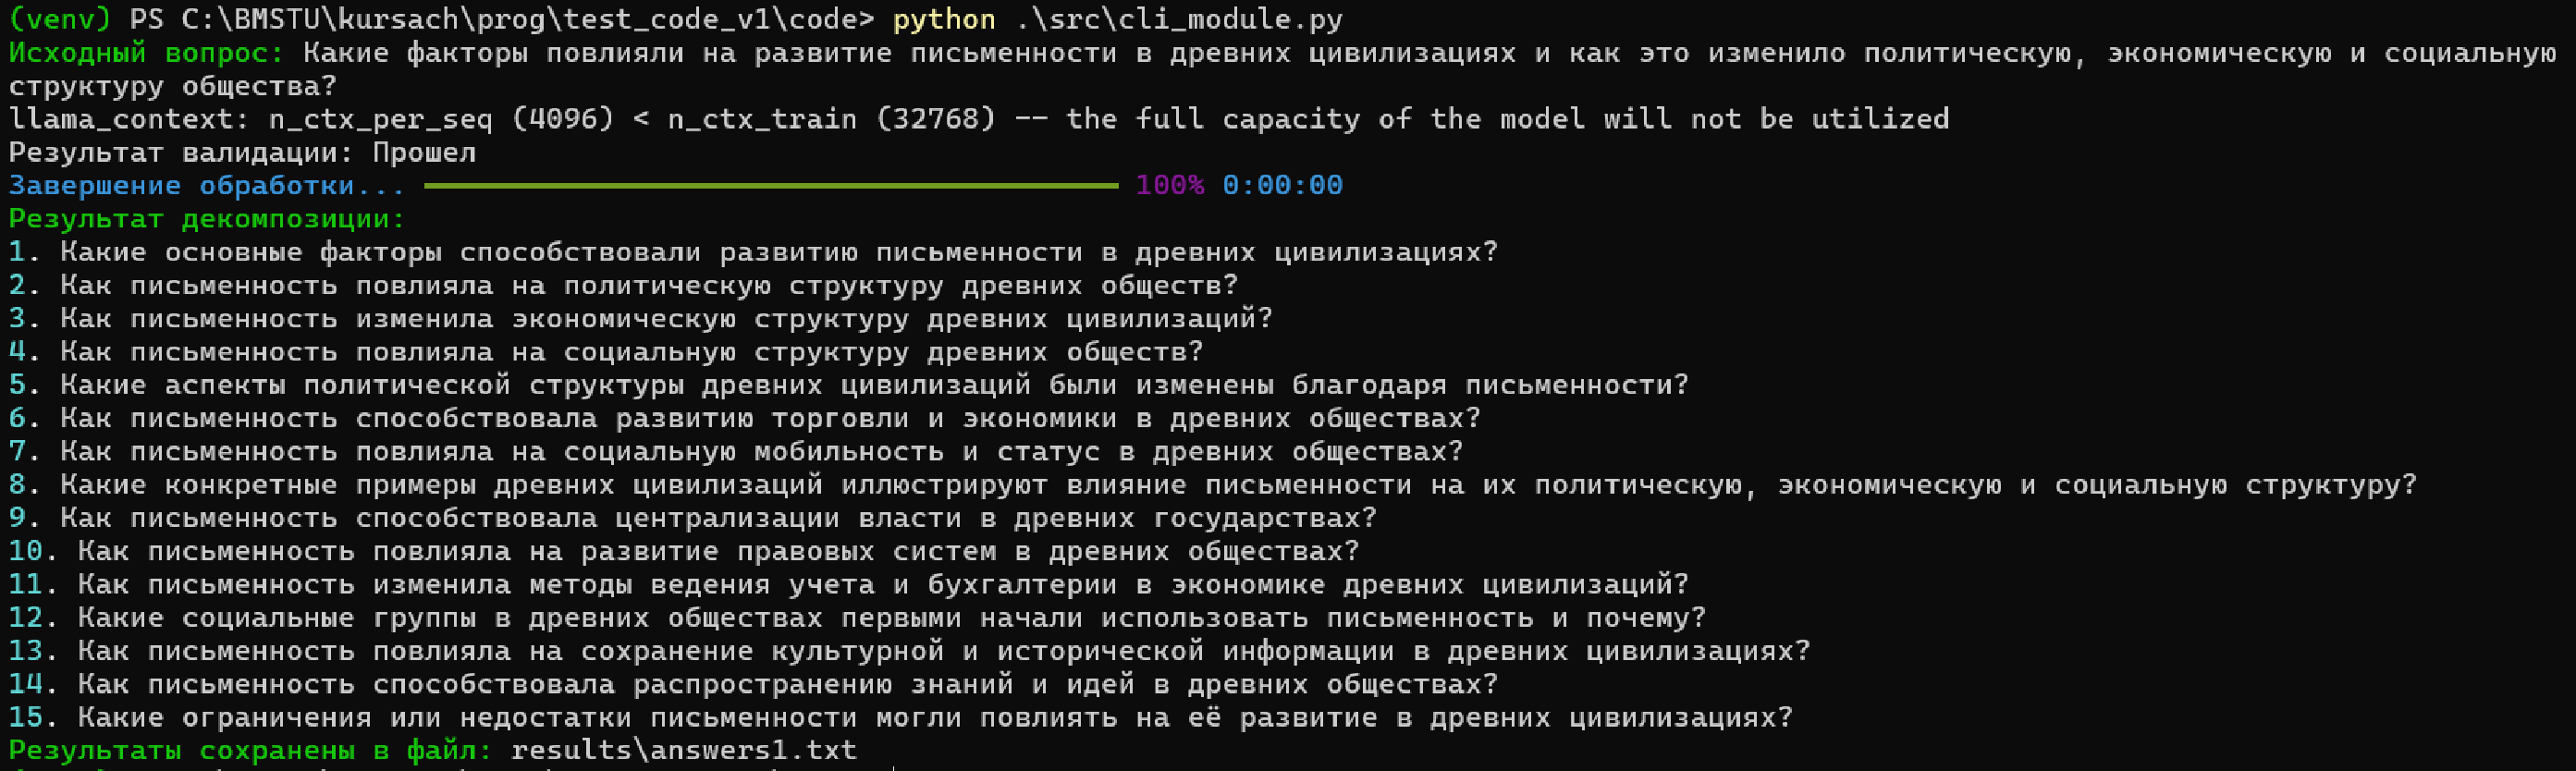
\includegraphics[width=1\textwidth]{images/program_execution.pdf}
\caption{Пример выполнения программы в командной строке}
\label{fig:program_execution}
\end{figure}

\section{Вывод}

В технологическом разделе представлена реализация программного решения для декомпозиции сложных вопросов на простые с использованием локальных языковых моделей.

Для разработки был выбран Python как основной язык программирования, что позволило эффективно использовать существующие библиотеки для работы с языковыми моделями. Решение разделено на три взаимосвязанных модуля: консольный интерфейс для взаимодействия с пользователем, управление запросами для формирования промптов и обработки ответов, и модуль работы с языковой моделью. Такое разделение упрощает понимание кода и дает возможность независимо модифицировать отдельные компоненты системы.

Программа поддерживает настройку через конфигурационные файлы, благодаря чему пользователь может менять параметры работы без изменения исходного кода. Особое внимание было уделено совместимости с разными устройствами -- система оптимизирована для работы на CPU, что исключает необходимость в графических ускорителях.

Важным дополнением к системе стал механизм валидации результатов, который проверяет соответствие ответов этическим и правовым нормам с помощью дополнительного запроса к той же языковой модели в роли эксперта. Эта функциональность дополнена системой проверки запрещенных слов, работающей на двух уровнях: входных запросов и генерируемых ответов. Это повышает надежность системы и минимизирует риски получения нежелательного контента.

К проекту прилагается подробная инструкция по установке и использованию, а также примеры декомпозиции сложных вопросов из разных областей знаний, демонстрирующие возможности системы. Улучшенная обработка ошибок с информативными сообщениями делает программу более дружественной к пользователю.

Созданное решение соответствует всем требованиям, определенным в предыдущих разделах работы. Система эффективно преобразует сложные вопросы в наборы простых компонентов, сохраняя при этом возможность дальнейшего развития функциональности благодаря модульной структуре.
	
	\chapter{Экспериментально-исследовательский раздел}

\section{Методология исследования}
Настоящее исследование направлено на сравнительный анализ языковых моделей применительно к задаче декомпозиции сложных вопросов. Основной фокус исследования — оценка качества декомпозиции и изучение практической применимости моделей в условиях ограниченных вычислительных ресурсов. В рамках исследования были проанализированы 30 языковых моделей, рассмотренных в аналитической части работы.

Необходимо отметить, что изначальный план исследования предполагал измерение времени обработки и потребления памяти моделями при выполнении декомпозиции. Однако в ходе работы выяснилось, что большинство рассмотренных в аналитическом разделе языковых моделей требует значительных вычислительных ресурсов, недоступных в рамках данного исследования. По этой причине основной акцент был сделан на экспертной оценке качества декомпозиции.

\subsection{Тестовая выборка}
Для проведения исследования была сформирована тестовая выборка из 10 сложных вопросов, охватывающих различные предметные области. Критериями отбора вопросов служили многокомпонентность (наличие нескольких аспектов, требующих рассмотрения), тематическое разнообразие и структурная сложность. Тестовая выборка представлена в таблице~\ref{tab:test-questions}.

\begin{table}[H]
	\caption{Тестовая выборка сложных вопросов}
	\label{tab:test-questions}
	\begin{tabular}{|p{0.5cm}|p{15.6cm}|}
		\hline
		\textbf{№} & \textbf{Вопрос} \\
		\hline
		1 & Какие факторы повлияли на развитие письменности в древних цивилизациях и как это изменило политическую, экономическую и социальную структуру общества? \\
		\hline
		2 & Как экологические проблемы, связанные с загрязнением океана пластиком, влияют на морских обитателей, прибрежные экосистемы и здоровье человека, и какие существуют технологические и законодательные решения для минимизации этого воздействия? \\
		\hline
		3 & Каково влияние искусственного интеллекта на рынок труда, образование и этические нормы общества, и как следует регулировать его развитие? \\
		\hline
		4 & Какие технологические прорывы в области квантовых вычислений могут изменить подход к криптографии и обработке больших данных в ближайшие десятилетия? \\
		\hline
		5 & Как глобализация повлияла на культурную идентичность малых народов и какие существуют стратегии сохранения языкового разнообразия? \\
		\hline
		6 & Какие медицинские, этические и юридические аспекты необходимо учитывать при внедрении генной инженерии в клиническую практику? \\
		\hline
		7 & Как развитие возобновляемых источников энергии изменяет геополитическую ситуацию и экономику стран-экспортеров нефти? \\
		\hline
		8 & Какие философские концепции лежат в основе современных подходов к искусственному интеллекту и как они влияют на его восприятие обществом? \\
		\hline
		9 & Какие нейробиологические механизмы ответственны за формирование долговременной памяти и как их понимание может помочь в лечении нейродегенеративных заболеваний? \\
		\hline
		10 & Как цифровизация образования влияет на когнитивное развитие студентов и какие риски она несет для традиционной педагогики? \\
		\hline
	\end{tabular}
\end{table}

\section{Оценка качества декомпозиции}
Оценка качества декомпозиции сложных вопросов проводилась экспертным методом. Для этого каждая из 30 исследуемых моделей использовалась для разбиения всех 10 вопросов из тестовой выборки. Полученные результаты анализировались квалифицированным экспертом с опытом в области лингвистики и обработки естественного языка.

С целью обеспечения объективности оценки был разработан комплекс критериев для стандартизации процесса экспертной оценки. Это позволило минимизировать субъективность и получить сопоставимые результаты для разных моделей.

\subsection{Критерии экспертной оценки}
Оценка качества декомпозиции проводилась по трем ключевым критериям:

\textbf{Полнота} (0-5 баллов): оценивает степень охвата всех смысловых аспектов исходного вопроса. Максимальный балл присваивался, если полученный набор подвопросов полностью покрывал информационную потребность исходного вопроса.

\textbf{Атомарность} (0-5 баллов): оценивает степень фокусировки каждого подвопроса на одном смысловом компоненте. Высокий балл присваивался, если подвопросы не содержали несколько разнородных аспектов и не требовали дальнейшей декомпозиции.

\textbf{Корректность} (0-5 баллов): оценивает грамматическую и логическую целостность подвопросов. Критерий учитывал логичность формулировок, отсутствие грамматических ошибок и стилистическую согласованность.

Процесс получения итоговой оценки включал два этапа усреднения. Сначала для каждой модели по каждому из трех критериев вычислялось среднее арифметическое оценок за все 10 тестовых вопросов. Затем полученные три средних значения (по полноте, атомарности и корректности) усреднялись, формируя итоговый показатель качества декомпозиции. Данный подход обеспечил комплексную оценку производительности моделей с учетом всех аспектов качества декомпозиции.

\subsection{Результаты оценки}
На основе анализа результатов декомпозиции 10 тестовых вопросов была составлена сводная таблица экспертных оценок по всем 30 исследуемым моделям (таблица~\ref{tab:expert-results-full}). Модели в таблице расположены в порядке убывания среднего балла.

\begin{table}[H]
	\caption{Сводные результаты экспертной оценки качества декомпозиции сложных вопросов}
	\label{tab:expert-results-full}
	\begin{tabular}{|l|B|B|B|B|}
		\hline
		\textbf{Модель} & \textbf{Полнота} & \textbf{Атомарность} & \textbf{Корректность} & \textbf{Средний балл} \\
		\hline
		DeepSeek-V3-Chat & 4.8 & 4.6 & 4.9 & 4.77 \\
		chatgpt-4o-latest & 4.7 & 4.5 & 4.8 & 4.67 \\
		claude-3-opus-20240229 & 4.4 & 4.5 & 4.7 & 4.53 \\
		o1-mini & 4.5 & 4.2 & 4.6 & 4.43 \\
		RuadaptQwen-32B-Pro\_v1 & 4.3 & 4.1 & 4.2 & 4.20 \\
		T-Tech-T-pro-it-1.0 & 4.2 & 4.1 & 4.3 & 4.20 \\
		yi-lightning & 4.3 & 4.1 & 4.2 & 4.20 \\
		gemini-1.5-pro-002 & 4.3 & 4.0 & 4.2 & 4.17 \\
		SberDevices-GigaChatMax & 4.0 & 4.3 & 4.0 & 4.10 \\
		Qwen2.5-72B-Instruct & 4.2 & 3.8 & 4.0 & 4.00 \\
		ru-Zero-Mistral-Small-24B & 3.9 & 4.0 & 4.1 & 4.00 \\
		Phi-4 & 3.9 & 3.7 & 4.3 & 3.97 \\
		llama-3.1-70b-instruct & 3.9 & 3.6 & 4.1 & 3.87 \\
		vikhr-nemo-12b-instruct-r & 3.8 & 4.0 & 3.8 & 3.87 \\
		mistral-large-2407 & 3.8 & 3.8 & 3.6 & 3.73 \\
		gemma-2-9b-it & 3.6 & 3.5 & 3.8 & 3.63 \\
		command-r-plus & 3.6 & 3.6 & 3.6 & 3.60 \\
		Watari-7b-v1 & 3.3 & 3.2 & 3.2 & 3.23 \\
		gpt-3.5-turbo-0125 & 2.9 & 3.5 & 3.1 & 3.17 \\
		MTSAIR-Cotype-Nano & 3.4 & 2.8 & 3.2 & 3.13 \\
		yandexgpt-4-pro & 3.2 & 3.1 & 3.1 & 3.13 \\
		glm-4-9b-chat & 2.9 & 2.8 & 3.1 & 2.93 \\
		c4ai-command-r-v01 & 2.7 & 2.8 & 2.7 & 2.73 \\
		hermes-2-theta-llama-3-8b & 2.6 & 2.7 & 2.8 & 2.70 \\
		suzume-llama-3-8b-multilingual & 2.7 & 2.6 & 2.8 & 2.70 \\
		saiga\_llama3\_8b\_v6 & 2.5 & 2.6 & 2.7 & 2.60 \\
		paralex-llama-3-8b-sft & 2.5 & 2.4 & 2.6 & 2.50 \\
		aya-23-8b & 2.4 & 2.3 & 2.5 & 2.40 \\
		storm-7b & 2.2 & 2.2 & 2.3 & 2.23 \\
		neural-chat-7b-v3-3 & 2.2 & 2.1 & 2.2 & 2.17 \\
		\hline
	\end{tabular}
\end{table}

\begin{figure}[H]
	\centering
	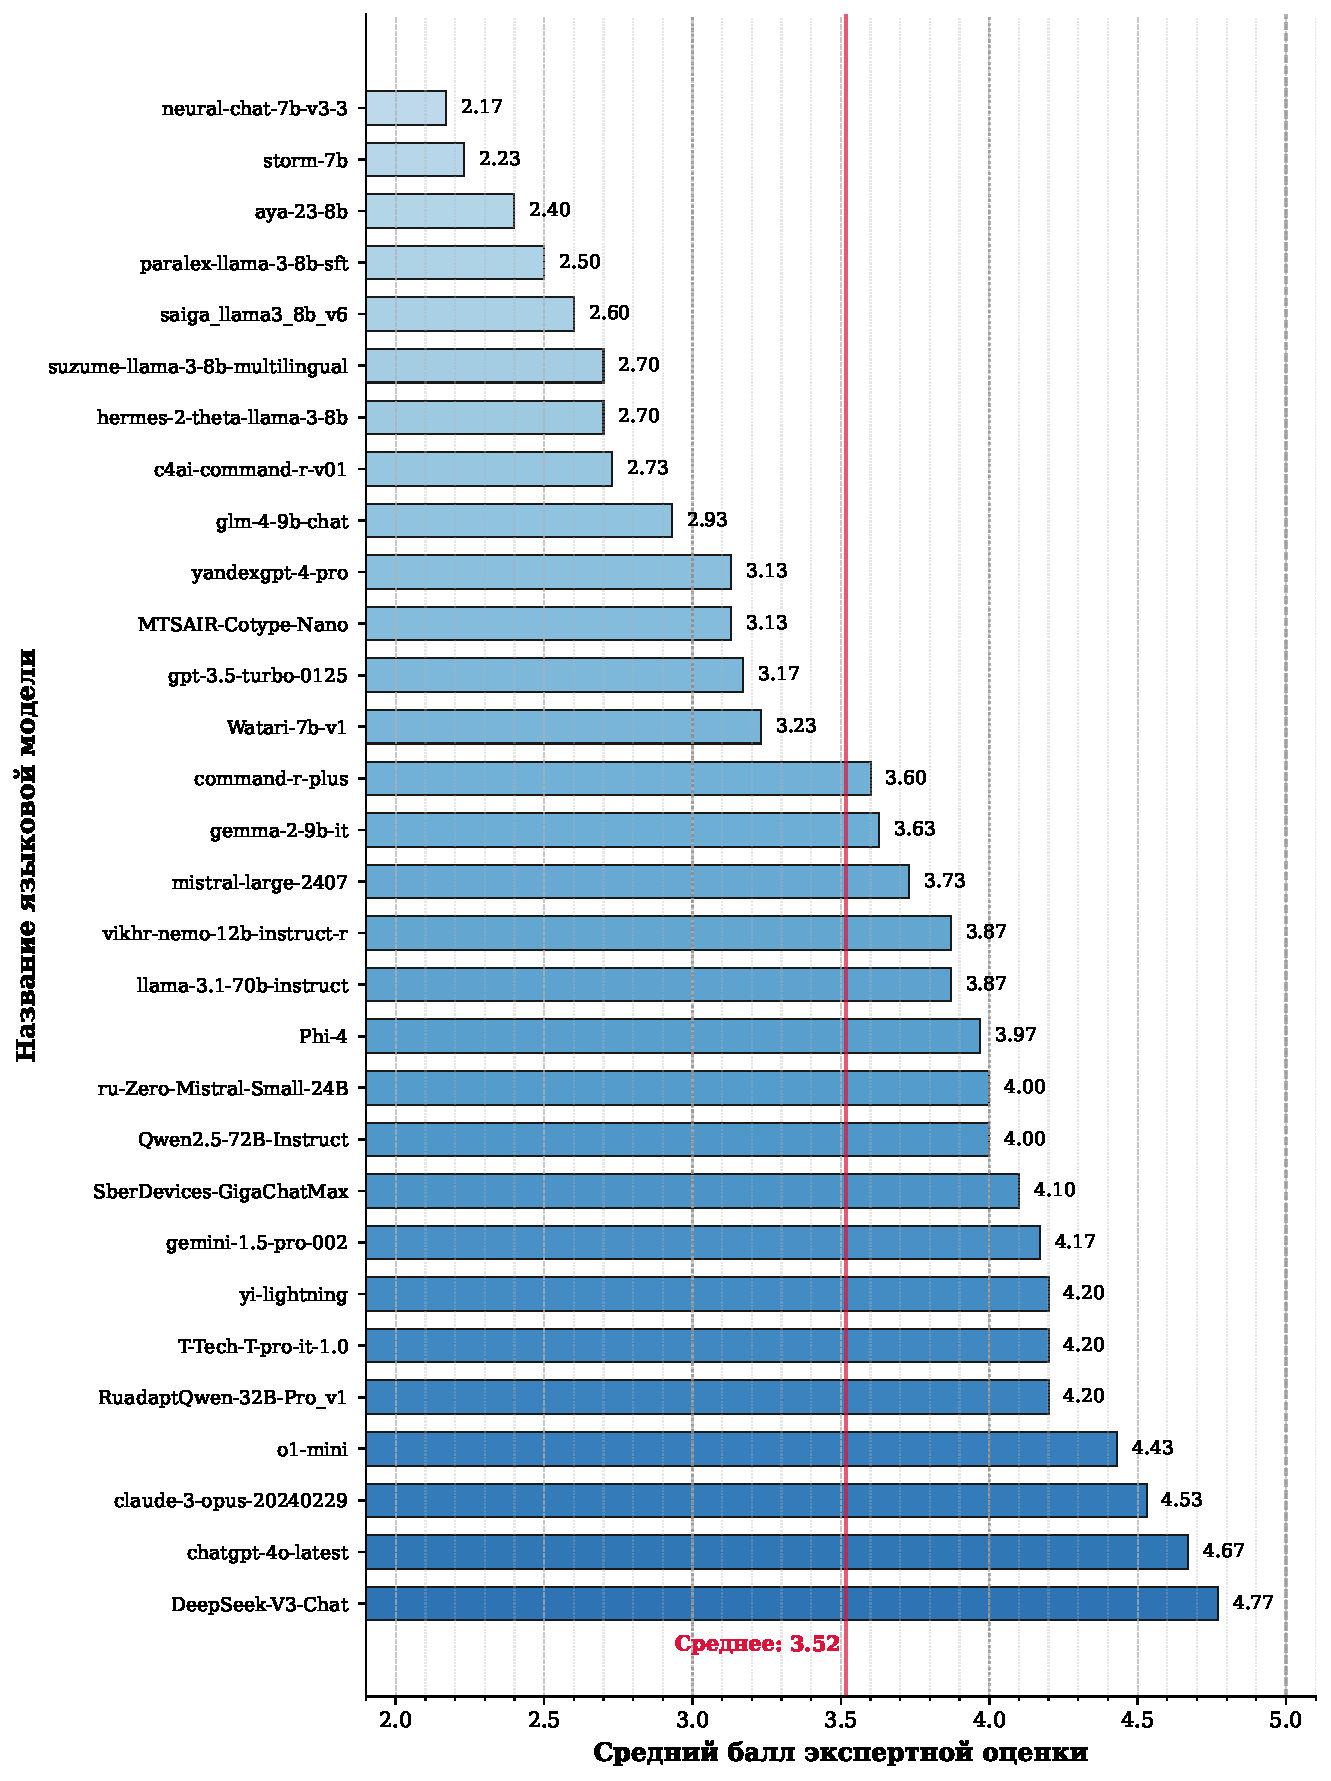
\includegraphics[width=1\textwidth]{images/model_performance_comparison.pdf}
	\caption{Сравнение моделей по интегральному показателю качества}
	\label{fig:quality}
\end{figure}

Проведенное исследование показало, что наилучшие результаты демонстрируют проприетарные модели DeepSeek-V3-Chat, chatgpt-4o-latest и Claude-3-Opus, доступные только через API. Среди локальных моделей высокие результаты показывают T-Tech-T-pro-it-1.0 и RuadaptQwen-32B-Pro\_v1 с показателем 4.20 балла, что подтверждает высокое качество этих открытых моделей.

\section{Практические ограничения}
Несмотря на значительное превосходство проприетарных моделей и крупных локальных моделей в качестве декомпозиции, их практическое применение сталкивается с серьезными ограничениями. Эти ограничения имеют существенное влияние на возможность проведения комплексного исследования всех аспектов работы моделей.

Анализ доступности моделей показал, что значительная часть решений с наивысшими показателями качества доступна исключительно через API, что делает невозможным их локальное развертывание. Такие модели как DeepSeek-V3-Chat, chatgpt-4o-latest, claude-3-opus, o1-mini, gemini-1.5-pro, SberDevices-GigaChatMax и другие могут использоваться только при наличии подключения к соответствующим сервисам и с учетом ограничений, устанавливаемых поставщиками этих сервисов.

Среди моделей, теоретически доступных для локального запуска, также существует значительное расслоение по требованиям к вычислительным ресурсам. Крупные модели, такие как LLaMA-3.1-70b-instruct (39.8 ГБ), Qwen2.5-72B (40.6 ГБ) и mistral-large-2407 (45.3 ГБ), требуют не менее 80-92 ГБ оперативной памяти, что существенно превышает возможности стандартных персональных компьютеров и требует специализированного серверного оборудования. Модели среднего размера, включая RuadaptQwen-32B (18.3 ГБ) и T-Tech-T-pro-it-1.0 (16.4 ГБ), хотя и требуют меньше ресурсов, всё равно выходят за рамки возможностей рядового пользовательского оборудования.

Данное ограничение не позволило провести полноценное исследование времени обработки и потребления памяти для большинства моделей, рассмотренных в аналитическом разделе, так как исследовательская среда имела в распоряжении только 8 ГБ оперативной памяти и не обладала специализированным графическим ускорителем, необходимым для эффективной работы крупных моделей.

Более того, сравнительный анализ компактных моделей (<10 ГБ), которые потенциально могли бы быть запущены в исследовательской среде, представляется малоинформативным по двум причинам. Во-первых, большинство таких моделей демонстрируют схожие характеристики производительности при работе на однотипном оборудовании, что обусловлено схожестью их архитектур и методов оптимизации. Во-вторых, детальное измерение производительности требует специализированных методик профилирования, позволяющих отделить собственно время инференса от операций пред- и постобработки текста, что выходит за рамки настоящего исследования.

Таким образом, основной фокус исследования был смещен в сторону оценки качества декомпозиции, которое может быть надежно измерено для всех моделей независимо от их доступности для локального запуска.

\subsection{Выбор модели для практической реализации}
Учитывая описанные выше ограничения и результаты экспертной оценки, для практической реализации системы декомпозиции вопросов была выбрана локальная квантованная модель T-lite-it-1.0-q4\_k\_m из семейства T Bank. Данный выбор обусловлен следующими факторами:

\begin{itemize}
	\item модель T-Tech-T-pro-it-1.0 из того же семейства продемонстрировала наилучшие результаты среди локальных моделей с оценкой 4.20 балла, что указывает на высокую эффективность архитектуры и обучения моделей этого семейства;
	
	\item несмотря на превосходные результаты, модель T-Tech-T-pro-it-1.0 требует 36 ГБ оперативной памяти, что превышает доступные ресурсы исследовательской среды;
	
	\item компактная модель T-lite-it-1.0-q4\_k\_m из того же семейства сохраняет базовые архитектурные особенности и обучающие данные, имея при этом существенно меньшие требования к ресурсам;
	
	\item размер модели составляет 4.68 ГБ, что позволяет запускать ее на стандартном персональном компьютере с ограниченными ресурсами;
	
	\item требуемый объем оперативной памяти не превышает 6 ГБ, что делает модель доступной для подавляющего большинства современных компьютеров;
	
	\item квантованная архитектура модели обеспечивает приемлемую скорость работы даже без использования графического ускорителя. \cite{t_lite_it_q4}
\end{itemize}


\section{Вывод}
Проприетарные модели, доступные через API, демонстрируют наивысшее качество декомпозиции сложных вопросов с оценками 4.77, 4.67 и 4.53 баллов для DeepSeek-V3-Chat, chatgpt-4o-latest и Claude-3-Opus соответственно. Однако их использование требует постоянного подключения к интернету и зависит от доступности и политики стороннего сервиса.

Среди локальных моделей наилучшие результаты показывает T-Tech-T-pro-it-1.0 с оценкой 4.20 баллов, что подтверждает высокое качество моделей семейства T Bank. Данная модель может считаться эталоном качества для решений, работающих без доступа к сети, однако требует значительных вычислительных ресурсов, недоступных на стандартных персональных компьютерах.

Квантованная модель T-lite-it-1.0-q4\_k\_m представляет собой оптимальный компромисс между качеством декомпозиции и возможностью запуска на потребительском оборудовании. Несмотря на более низкий показатель качества по сравнению с проприетарными решениями, модель обеспечивает приемлемый уровень декомпозиции и может быть успешно использована в практических приложениях.

Таким образом, исследование показало возможность эффективной декомпозиции сложных вопросов с использованием языковых моделей различного масштаба, что открывает перспективы для создания практических приложений, способных работать в условиях ограниченных вычислительных ресурсов.
	
	\chapter{Организационно-правовой раздел}

\section{Лицензионная политика проекта}

Программное решение распространяется под лицензией Apache 2.0 \cite{apache}, что обусловлено требованиями используемой языковой модели T-lite-it-1.0 \cite{tlite} от T Bank и необходимостью обеспечения совместимости с компонентами, лицензированными под MIT \cite{mit}.

\subsection{Обоснование выбора лицензии}

Проект включает библиотеки \texttt{typer} \cite{typer}, \texttt{pydantic} \cite{pydantic}, \texttt{rich} \cite{rich} и \texttt{llama-cpp-python} \cite{llama-cpp-python}, распространяемые под лицензией MIT. Совместимость лицензий MIT и Apache 2.0 подтверждается сравнительным анализом их требований (табл.~\ref{tab:license-comparison}). Текст лицензии Apache 2.0 находится в приложении A.

\begin{table}[ht]
	\centering
	\caption{Сравнительный анализ лицензий MIT и Apache 2.0}
	\label{tab:license-comparison}
	\begin{tabular}{|p{4.5cm}|p{3.5cm}|p{3.5cm}|p{2.5cm}|}
		\hline
		\textbf{Критерий} & \textbf{Лицензия MIT} & \textbf{Лицензия Apache 2.0} & \textbf{Сравнение} \\
		\hline
		Коммерческое использование & Разрешено & Разрешено & Одинаково \\
		\hline
		Модификация & Разрешено без ограничений & Разрешено с требованием указания изменений & Apache 2.0 строже \\
		\hline
		Распространение & Разрешено & Разрешено с дополнительными требованиями & Apache 2.0 строже \\
		\hline
		Частное использование & Разрешено & Разрешено & Одинаково \\
		\hline
		Указание изменений & Не требуется явно & Требуется явное указание & Apache 2.0 строже \\
		\hline
		Защита авторских прав & Требует включения уведомления & Требует сохранения всех уведомлений & Apache 2.0 строже \\
		\hline
		Патентные права & Нет явного предоставления & Явное предоставление патентных прав & Apache 2.0 строже \\
		\hline
		Ограничение торговых марок & Отсутствует & Прямо запрещает использование & Apache 2.0 строже \\
		\hline
		Распространение производных & Разрешено без особых условий & Разрешено с дополнительными условиями & Apache 2.0 строже \\
		\hline
	\end{tabular}
\end{table}

\subsection{Правовые аспекты использования лицензии}

Анализ таблицы~\ref{tab:license-comparison} показывает, что Apache 2.0 по всем критериям либо эквивалентна MIT, либо накладывает более строгие ограничения. Согласно принципам лицензионной совместимости, подтвержденным \mbox{Open Source Initiative \cite{osi}}, компоненты с более открытой лицензией (MIT) могут включаться в проекты под более строгой лицензией (Apache 2.0) при соблюдении требований обеих лицензий.

Ключевые преимущества выбранной лицензионной политики:

\begin{itemize}
	\item правовая защита посредством явного предоставления патентных прав;
	\item чёткие требования к указанию модификаций, обеспечивающие прозрачность изменений;
	\item сохранение авторских прав разработчиков;
	\item возможность коммерческого использования с соблюдением условий лицензии.
\end{itemize}

Для учебных целей применение программного решения дополнительно защищено ст. 1274 ГК РФ, разрешающей свободное использование объектов авторского права в образовательном процессе.

\section{Меры правовой безопасности}

\subsection{Многоуровневая валидация контента}
Фильтрация контента обязательна согласно ст. 10.1 ФЗ-149 <<Об информации, информационных технологиях и о защите информации>>, требующей блокировки запрещённой информации (экстремизм, призывы к насилию), а также ФЗ-114 <<О противодействии экстремистской деятельности>>. Несоблюдение влечёт ответственность по ст. 282 УК РФ и ст. 13.41 КоАП РФ, а также риск блокировки проекта.

Архитектура системы включает комплексный подход к обеспечению правовой безопасности, сочетающий жёсткую и мягкую фильтрацию контента:

\begin{enumerate}
	\item \textbf{жёсткая фильтрация} основана на автоматической проверке текста по спискам запрещённых слов и словосочетаний, формируемым на основе официальных источников:
	\begin{itemize}
		\item список экстремистских материалов Министерства юстиции РФ \cite{minust};
		\item единый реестр запрещенной информации Роскомнадзора \cite{rkn};
		\item перечень запрещённой информации согласно постановлениям Верховного Суда РФ \cite{verh_sud};
		\item список экстремистских и террористических организаций, признанных таковыми Генеральной прокуратурой РФ \cite{prokur};
		\item рекомендации Минцифры \cite{min_cifr}.
	\end{itemize}
	
	\item \textbf{мягкая фильтрация} реализуется посредством нейросетевой модели, которая:
	\begin{itemize}
		\item на этапе предварительной обработки получает системные инструкции с явными запретами на генерацию контента, нарушающего законодательство РФ, включая ст. 282 УК РФ, ФЗ-149;
		\item выполняет семантический анализ содержания, способный идентифицировать противоправный контент даже при использовании эвфемизмов или нестандартных формулировок.
	\end{itemize}
\end{enumerate}

На этапе постобработки ответ модели анализируется через дополнительный валидационный запрос. При обнаружении потенциальных нарушений система блокирует выдачу контента и прекращает обработку запроса.

\subsection{Формирование и обновление списков запрещённых слов}
Базовые списки запрещённых слов и выражений формируются на основе официальных источников регулирующих органов РФ, которые были указаны выше.

\textbf{Обязанность пользователя:} В соответствии с требованиями ст. 10.1 \mbox{ФЗ-149}, пользователь несёт полную ответственность за:

\begin{itemize}
	\item регулярное обновление встроенных списков запрещённых слов и выражений из вышеуказанных официальных источников, в соответствии с изменениями в действующем законодательстве;
	\item самостоятельное дополнение базовых списков с учётом специфики использования программы и отраслевых требований;
	\item проверку актуальности используемых фильтров перед каждым применением программного решения.
\end{itemize}

Система предоставляет техническую возможность для обновления списков, но \textbf{не осуществляет их автоматическое обновление}. Вся ответственность за актуальность и полноту списков запрещённых слов и выражений лежит исключительно на пользователе программного решения.

\subsection{Обработка персональных данных}
В соответствии с требованиями ФЗ-152 <<О персональных данных>> и \mbox{ФЗ-149} <<Об информации, информационных технологиях и о защите информации>>:

\begin{itemize}
	\item программное решение \textbf{не предназначено} для обработки персональных данных и \textbf{не должно использоваться} для этих целей;
	\item система настроена на блокировку генерации и обработки контента, содержащего персональные данные;
	\item \textbf{пользователю категорически запрещается} вводить персональные данные субъектов в систему;
	\item в случае ввода персональных данных в систему вся ответственность за их обработку в соответствии со ст. 13.11 КоАП РФ и ФЗ-152 возлагается исключительно на пользователя.
\end{itemize}

При обнаружении в запросе признаков персональных данных система предупреждает пользователя о недопустимости их обработки и может отказать в выполнении запроса.

\subsection{Ответственность пользователя}
Перед каждым использованием программы пользователь обязан:
\begin{itemize}
	\item самостоятельно убедиться в актуальности используемых списков запрещённых слов и выражений путём проверки официальных источников;
	\item обновить базы данных запрещённых выражений в соответствии с изменениями в законодательстве;
	\item дополнить систему фильтрации собственными ограничениями в соответствии с конкретными задачами использования системы;
	\item верифицировать результаты работы системы на соответствие действующему законодательству РФ.
\end{itemize}

\newpage
В соответствии с ст. 13.41 КоАП РФ и общими положениями гражданского законодательства, пользователь несёт полную юридическую ответственность за:
\begin{itemize}
	\item актуальность и полноту используемых фильтров запрещённой информации;
	\item недопущение обработки персональных данных с использованием системы;
	\item использование и распространение информации, полученной с помощью данного программного обеспечения.
\end{itemize}

Разработчик не несёт ответственности за последствия использования программы в нарушение действующего законодательства, несмотря на наличие встроенных механизмов защиты.

\subsection{Ограничения и риски}
Система подвержена следующим технико-правовым ограничениям: появление ложных срабатываний при обработке специализированных научных, медицинских и юридических терминов; возможность обхода фильтров через сложные лингвистические конструкции; недостаточная точность интерпретации контекста при анализе многозначных выражений. Эффективность фильтрации зависит от регулярности обновления пользователем баз запрещённых выражений в соответствии с изменениями законодательства.

\section{Вывод}
Реализованные правовые механизмы обеспечивают соответствие проекта требованиям ФЗ-149, ФЗ-114 и УК РФ за счёт многоуровневой фильтрации контента, основанной на официальных списках запрещённых материалов и нейросетевом анализе. Лицензия Apache 2.0 гарантирует совместимость с компонентами MIT, а распределение ответственности (обновление фильтров, запрет на обработку персональных данных) минимизирует юридические риски.
	
	\phantomsection
\part*{ЗАКЛЮЧЕНИЕ}
\addcontentsline{toc}{chapter}{\textbf{ЗАКЛЮЧЕНИЕ}}

В рамках курсового проекта разработано программное решение для автоматической декомпозиции сложных вопросов на простые с использованием больших языковых моделей. 

Анализ существующих подходов показал преимущества применения языковых моделей над экспертными и алгоритмическими методами: отсутствие необходимости в разработке сложных правил, высокая адаптивность к различным типам вопросов и эффективное сохранение контекста между частями исходного вопроса.

Разработанная архитектура включает три взаимосвязанных модуля: консольный интерфейс, управление запросами и взаимодействие с языковой моделью. Реализация на Python обеспечивает работу на стандартном оборудовании без необходимости в графических ускорителях. Внедрена двухуровневая система валидации контента для входных запросов и генерируемых ответов.

Экспериментальное исследование выявило, что проприетарные модели (DeepSeek-V3-Chat, ChatGPT-4, Claude-3-Opus) демонстрируют наивысшее качество декомпозиции, однако требуют постоянного подключения к интернету. Среди локальных решений выделяются T-Tech-T-pro-it-1.0 и RuadaptQwen-32B-Pro\_v1. Для практической реализации выбрана компактная квантованная модель T-lite-it-1.0-q4\_k\_m как оптимальный компромисс между качеством и доступностью на пользовательском оборудовании.

Программное решение распространяется под лицензией Apache 2.0 и соответствует требованиям законодательства РФ благодаря реализованной фильтрации контента на основе официальных источников.

В результате созданное программное решение успешно выполняет декомпозицию сложных вопросов на простые компоненты и может применяться в образовательных системах, системах поддержки принятия решений и других приложениях обработки естественного языка.
	
	\phantomsection
	\printbibliography[
	title=\centerline{СПИСОК ИСПОЛЬЗОВАННЫХ ИСТОЧНИКОВ}
	]
	\addcontentsline{toc}{chapter}{\textbf{СПИСОК ИСПОЛЬЗОВАННЫХ ИСТОЧНИКОВ}}
	
	\phantomsection
\stepcounter{appendix}
\chapter*{\centerline{ПРИЛОЖЕНИЕ \Asbuk{appendix}}}
\addcontentsline{toc}{chapter}{\textbf{ПРИЛОЖЕНИЕ \Asbuk{appendix}}}

                                 Apache License
Version 2.0, January 2004
http://www.apache.org/licenses/

TERMS AND CONDITIONS FOR USE, REPRODUCTION, AND DISTRIBUTION

1. Definitions.

"License" shall mean the terms and conditions for use, reproduction,
and distribution as defined by Sections 1 through 9 of this document.

"Licensor" shall mean the copyright owner or entity authorized by
the copyright owner that is granting the License.

"Legal Entity" shall mean the union of the acting entity and all
other entities that control, are controlled by, or are under common
control with that entity. For the purposes of this definition,
"control" means (i) the power, direct or indirect, to cause the
direction or management of such entity, whether by contract or
otherwise, or (ii) ownership of fifty percent (50%) or more of the
outstanding shares, or (iii) beneficial ownership of such entity.

"You" (or "Your") shall mean an individual or Legal Entity
exercising permissions granted by this License.

"Source" form shall mean the preferred form for making modifications,
including but not limited to software source code, documentation
source, and configuration files.

"Object" form shall mean any form resulting from mechanical
transformation or translation of a Source form, including but
not limited to compiled object code, generated documentation,
and conversions to other media types.

"Work" shall mean the work of authorship, whether in Source or
Object form, made available under the License, as indicated by a
copyright notice that is included in or attached to the work
(an example is provided in the Appendix below).

"Derivative Works" shall mean any work, whether in Source or Object
form, that is based on (or derived from) the Work and for which the
editorial revisions, annotations, elaborations, or other modifications
represent, as a whole, an original work of authorship. For the purposes
of this License, Derivative Works shall not include works that remain
separable from, or merely link (or bind by name) to the interfaces of,
the Work and Derivative Works thereof.

"Contribution" shall mean any work of authorship, including
the original version of the Work and any modifications or additions
to that Work or Derivative Works thereof, that is intentionally
submitted to Licensor for inclusion in the Work by the copyright owner
or by an individual or Legal Entity authorized to submit on behalf of
the copyright owner. For the purposes of this definition, "submitted"
means any form of electronic, verbal, or written communication sent
to the Licensor or its representatives, including but not limited to
communication on electronic mailing lists, source code control systems,
and issue tracking systems that are managed by, or on behalf of, the
Licensor for the purpose of discussing and improving the Work, but
excluding communication that is conspicuously marked or otherwise
designated in writing by the copyright owner as "Not a Contribution."

"Contributor" shall mean Licensor and any individual or Legal Entity
on behalf of whom a Contribution has been received by Licensor and
subsequently incorporated within the Work.

2. Grant of Copyright License. Subject to the terms and conditions of
this License, each Contributor hereby grants to You a perpetual,
worldwide, non-exclusive, no-charge, royalty-free, irrevocable
copyright license to reproduce, prepare Derivative Works of,
publicly display, publicly perform, sublicense, and distribute the
Work and such Derivative Works in Source or Object form.

3. Grant of Patent License. Subject to the terms and conditions of
this License, each Contributor hereby grants to You a perpetual,
worldwide, non-exclusive, no-charge, royalty-free, irrevocable
(except as stated in this section) patent license to make, have made,
use, offer to sell, sell, import, and otherwise transfer the Work,
where such license applies only to those patent claims licensable
by such Contributor that are necessarily infringed by their
Contribution(s) alone or by combination of their Contribution(s)
with the Work to which such Contribution(s) was submitted. If You
institute patent litigation against any entity (including a
cross-claim or counterclaim in a lawsuit) alleging that the Work
or a Contribution incorporated within the Work constitutes direct
or contributory patent infringement, then any patent licenses
granted to You under this License for that Work shall terminate
as of the date such litigation is filed.

4. Redistribution. You may reproduce and distribute copies of the
Work or Derivative Works thereof in any medium, with or without
modifications, and in Source or Object form, provided that You
meet the following conditions:

(a) You must give any other recipients of the Work or
Derivative Works a copy of this License; and

(b) You must cause any modified files to carry prominent notices
stating that You changed the files; and

(c) You must retain, in the Source form of any Derivative Works
that You distribute, all copyright, patent, trademark, and
attribution notices from the Source form of the Work,
excluding those notices that do not pertain to any part of
the Derivative Works; and

(d) If the Work includes a "NOTICE" text file as part of its
distribution, then any Derivative Works that You distribute must
include a readable copy of the attribution notices contained
within such NOTICE file, excluding those notices that do not
pertain to any part of the Derivative Works, in at least one
of the following places: within a NOTICE text file distributed
as part of the Derivative Works; within the Source form or
documentation, if provided along with the Derivative Works; or,
within a display generated by the Derivative Works, if and
wherever such third-party notices normally appear. The contents
of the NOTICE file are for informational purposes only and
do not modify the License. You may add Your own attribution
notices within Derivative Works that You distribute, alongside
or as an addendum to the NOTICE text from the Work, provided
that such additional attribution notices cannot be construed
as modifying the License.

You may add Your own copyright statement to Your modifications and
may provide additional or different license terms and conditions
for use, reproduction, or distribution of Your modifications, or
for any such Derivative Works as a whole, provided Your use,
reproduction, and distribution of the Work otherwise complies with
the conditions stated in this License.

5. Submission of Contributions. Unless You explicitly state otherwise,
any Contribution intentionally submitted for inclusion in the Work
by You to the Licensor shall be under the terms and conditions of
this License, without any additional terms or conditions.
Notwithstanding the above, nothing herein shall supersede or modify
the terms of any separate license agreement you may have executed
with Licensor regarding such Contributions.

6. Trademarks. This License does not grant permission to use the trade
names, trademarks, service marks, or product names of the Licensor,
except as required for reasonable and customary use in describing the
origin of the Work and reproducing the content of the NOTICE file.

7. Disclaimer of Warranty. Unless required by applicable law or
agreed to in writing, Licensor provides the Work (and each
Contributor provides its Contributions) on an "AS IS" BASIS,
WITHOUT WARRANTIES OR CONDITIONS OF ANY KIND, either express or
implied, including, without limitation, any warranties or conditions
of TITLE, NON-INFRINGEMENT, MERCHANTABILITY, or FITNESS FOR A
PARTICULAR PURPOSE. You are solely responsible for determining the
appropriateness of using or redistributing the Work and assume any
risks associated with Your exercise of permissions under this License.

8. Limitation of Liability. In no event and under no legal theory,
whether in tort (including negligence), contract, or otherwise,
unless required by applicable law (such as deliberate and grossly
negligent acts) or agreed to in writing, shall any Contributor be
liable to You for damages, including any direct, indirect, special,
incidental, or consequential damages of any character arising as a
result of this License or out of the use or inability to use the
Work (including but not limited to damages for loss of goodwill,
work stoppage, computer failure or malfunction, or any and all
other commercial damages or losses), even if such Contributor
has been advised of the possibility of such damages.

9. Accepting Warranty or Additional Liability. While redistributing
the Work or Derivative Works thereof, You may choose to offer,
and charge a fee for, acceptance of support, warranty, indemnity,
or other liability obligations and/or rights consistent with this
License. However, in accepting such obligations, You may act only
on Your own behalf and on Your sole responsibility, not on behalf
of any other Contributor, and only if You agree to indemnify,
defend, and hold each Contributor harmless for any liability
incurred by, or claims asserted against, such Contributor by reason
of your accepting any such warranty or additional liability.

END OF TERMS AND CONDITIONS

APPENDIX: How to apply the Apache License to your work.

To apply the Apache License to your work, attach the following
boilerplate notice, with the fields enclosed by brackets "[]"
replaced with your own identifying information. (Don't include
the brackets!)  The text should be enclosed in the appropriate
comment syntax for the file format. We also recommend that a
file or class name and description of purpose be included on the
same "printed page" as the copyright notice for easier
identification within third-party archives.

Copyright [yyyy] [name of copyright owner]

Licensed under the Apache License, Version 2.0 (the "License");
you may not use this file except in compliance with the License.
You may obtain a copy of the License at

http://www.apache.org/licenses/LICENSE-2.0

Unless required by applicable law or agreed to in writing, software
distributed under the License is distributed on an "AS IS" BASIS,
WITHOUT WARRANTIES OR CONDITIONS OF ANY KIND, either express or implied.
See the License for the specific language governing permissions and
limitations under the License.


\newpage
\stepcounter{appendix}  % увеличиваем счетчик приложений
\chapter*{\centerline{ПРИЛОЖЕНИЕ \Asbuk{appendix}}}
\addcontentsline{toc}{part}{\textbf{ПРИЛОЖЕНИЕ \Asbuk{appendix}}}

Презентация, состоящая из 17 слайдов.
	
	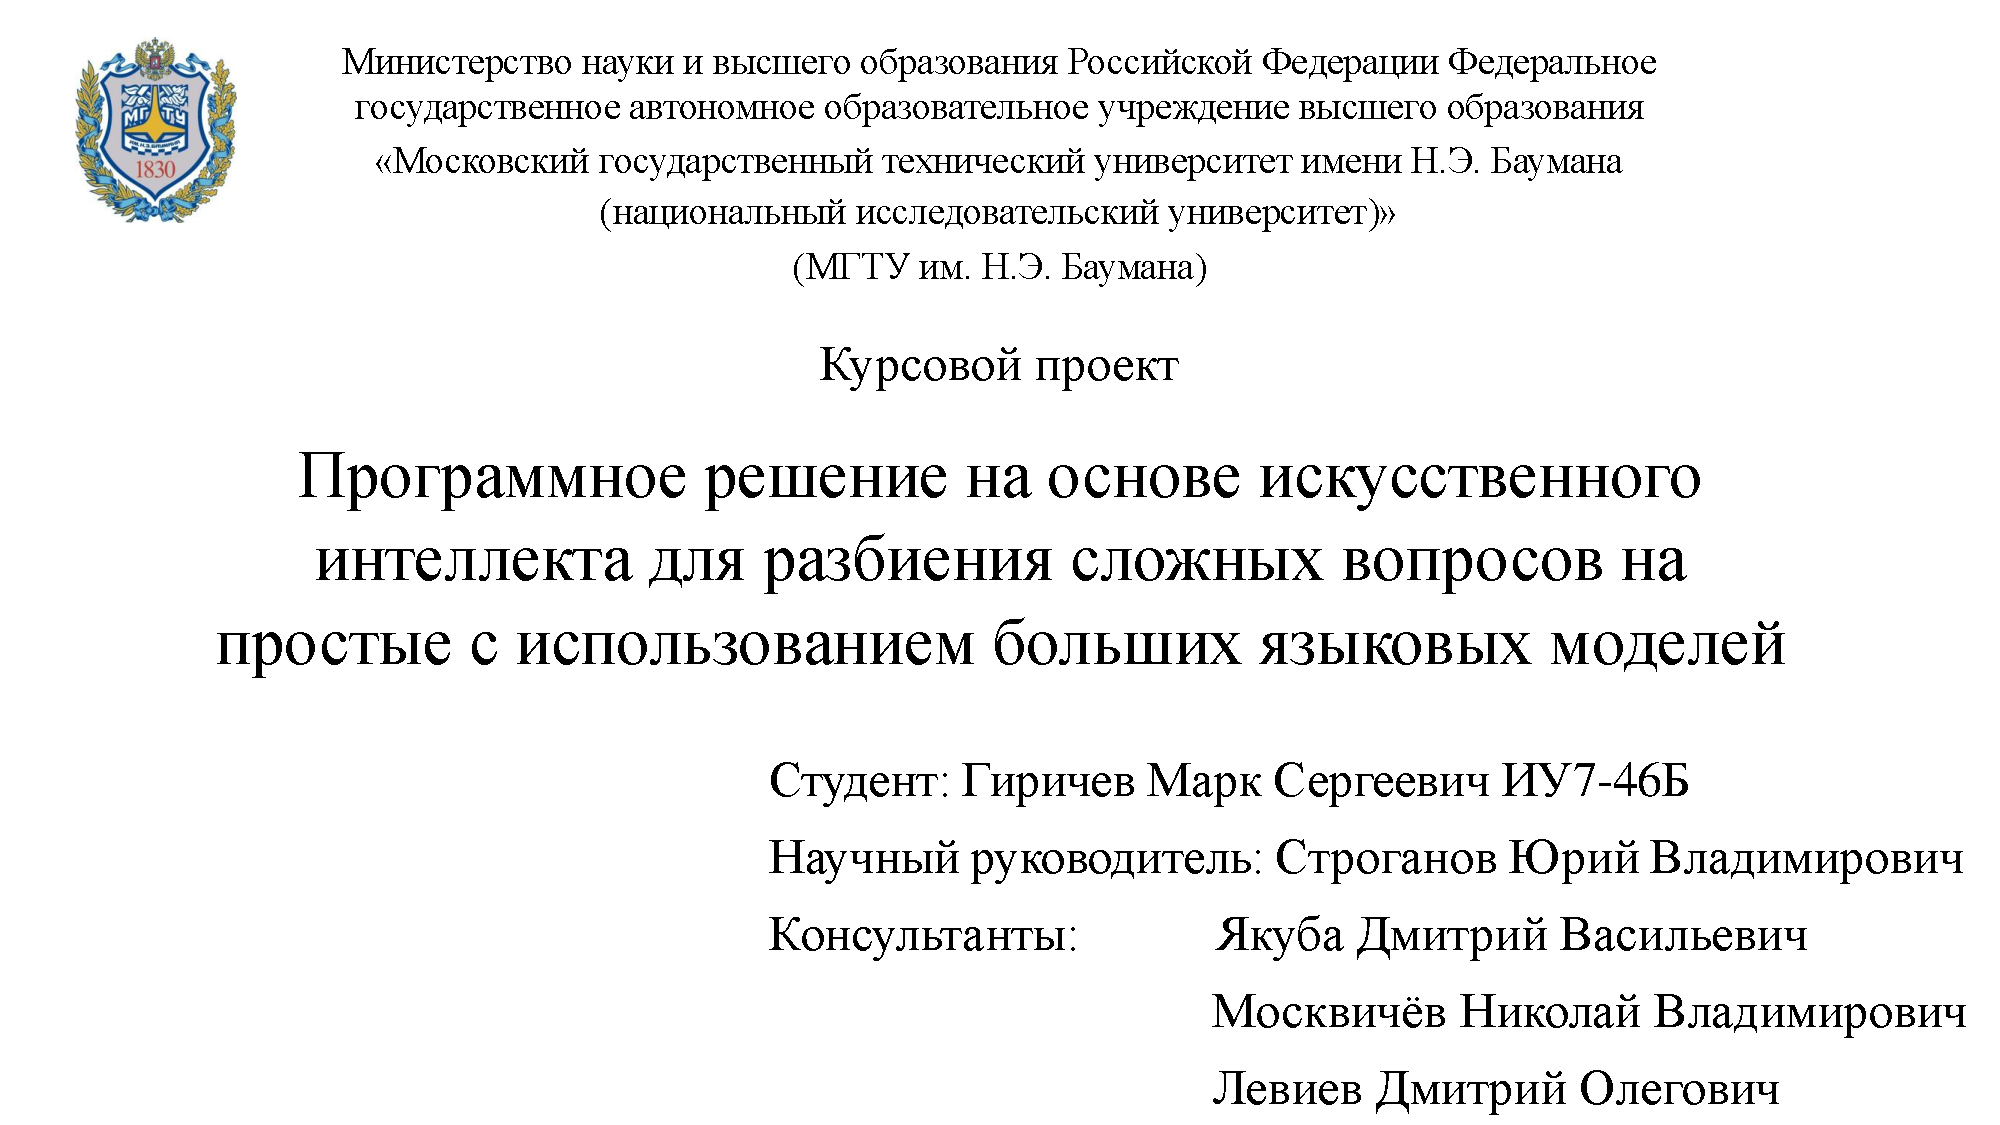
\includepdf[pages=-,angle=90]{presentation.pdf}

\end{document}
